%!TEX root = vivek-talk.tex 

\begin{frame}[label=apptuningovw]{Application Performance Tuning}{An Overview}
\begin{itemize}
    \item Performance Tuning of Computer Program Simulating Plasma-Coupled Combustion.
    \item Performance Tuning of 3-dimensional Image reconstruction of integrated circuits for finding intentional or unintentional defects in the circuits.
    \item Performance Tuning Communication-Avoiding Dense Matrix Factorizations. 
\end{itemize}
\end{frame}
%\begin{frame}{The Need to Simulate of Plasma Combustion}
%\end{frame} 

\begin{frame}[label=workWithGPUs]
  \frametitle{Efficient Simulation of Plasma Combustion of Clusters of GPUs}
  \begin{itemize}
  \small \item \small The Need to Simulate of Plasma Combustion. 
  \item \small Working with scientists in physics and mechanical sciences to integrate my techniques in a real-world CFD application for Plasma Combustion.
  \item \small Apply work in the context of heterogeneous architectures.
  \item \small Use loop scheduling ideas on MIC.
  \item \small Functionized vs non-functionized code
  \item \small GPU fraction
  \end{itemize}
\end{frame}

%!TEX root = schedCompPres.tex 

% General Goal: I want you to add this into your scheduling
% strategies.  
% General Goal: Tell audience that what I'm doing is relevant. 
% Specific Goal: Tell audience that low-overhead scheduling can
% benefit the energy efficiency for the product/application that you
% are creating - making money for the company. 

% TODO:L5: Practice presentation. 

% TODO: L4: Write presentation transitions 

% TODO: L4: Decide what to do for the application program timelines.
% -done 

% TODO:L0: add motivation for scheduler composition. - done 

% TODO:L4: Fix slide on schedulers. 

% TODO: L0: add experimental setup =  - done 
% TODO: L0: add descriptions for each scheduler  
%TODO:L3: check numbering and consistency 
%TODO: think about how to present snap 
%TODO: go through transitions and practice in morning 
%TODO: think about title 
%TODO: check that sentence comes at beginning. 
%TODO: add in a proper stencil code
\comments{
\begin{frame} 
\frametitle{Using Threading for PlasComCM}
\begin{center} 
{\tiny Insert 4 OpenMP low-overhead scheduling slides here.}
\end{center} 
\end{frame} 
}

\comments{
  \begin{frame}[label=lastslide]
    \frametitle{Current Work with GPUs}
    \begin{itemize}
      \item Working with scientists in physics and mechanical sciences to integrate my techniques in a real-world CFD application.
      \item Apply work in the context of heterogeneous
        architectures. 
       \item Use loop scheduling ideas on MIC. 
    \end{itemize}
  \end{frame}
}

\begin{frame}[label=synchMPICode]
\frametitle{Sample MPI Code} 
%common pattern 
\visible<1->{\small Common pattern in application codes.\\
% e.g., in~\hyperlink{appCodesAndSetup}{ones}\comments{\hyperlink{}{SNAP}, \hyperlink{}{miniFE}, \hyperlink{}{Rebound},} we'll see later.\comments{, we'll see
%in the experimentation section later.}
}
%\visible<1->{\lstinputlisting{./listings/mpi-bulk-synch.c}}
%\visible<1->{\lstinputlisting{./listings/MPIstencil.c}}
%\visible<2->{\lstinputlisting{./listings/mpi-synch-code-inst.c}} 
\vspace{0.1in}
\visible<1->{\small Assuming this code is perfectly load balanced,
  should be no performance problems.}
\end{frame}

\comments{
\begin{frame}[label=transImbMitigation]
  \frametitle{Transient Load Imbalance and its Mitigation}
  \begin{columns}
    \column{0.5\columnwidth}
    \visible<1->{\small Infrequent noise $\rightarrow$ slowdown at
      scale.}
    %TODO: slowdown?                                                  
    \column{0.5\columnwidth}
    \visible<1->{{\small \comments{$\exists$ large \# cores / node
          $\rightarrow$}Idea for fix: redistribute within node.}}
  \end{columns}
  %TODO: animate this to show  right one slide later.     
%  \visible<1->{
%    \begin{figure}[ht!]
%      \label{fig:NoiseTransImbPic}
%      \label{fig:AmplificationPic1}\subfloat[\label{fig:AmplificationPic1}
%        \tiny Noise\comments{different nodes in different iterations}
%        delays almost every
%        iteration.]{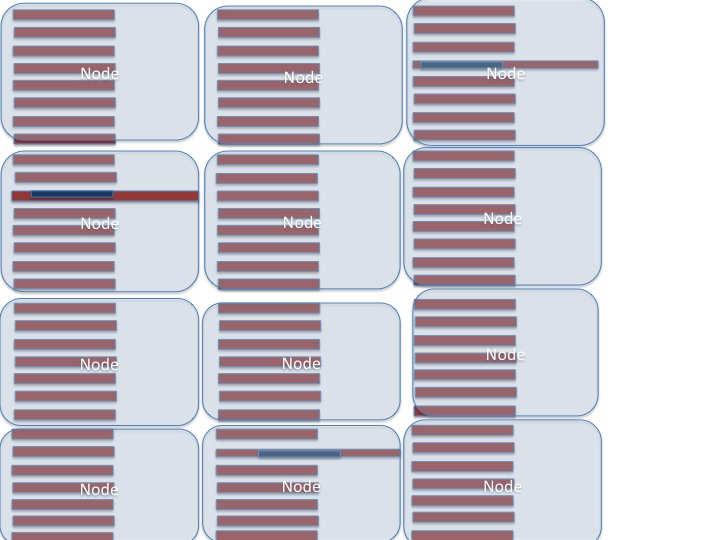
\includegraphics[height=1.3in]{./pictures/Noise}}}\visible<1->{\label{fig:AmplificationPic3}\hspace*{0.25in}\subfloat[\label{fig:AmplificationPic3}{\tiny
%        Performance improves, assuming perfect work re-distribution within each node. } %can be perfectly
      %re-distributed within each node.                        
%  ]{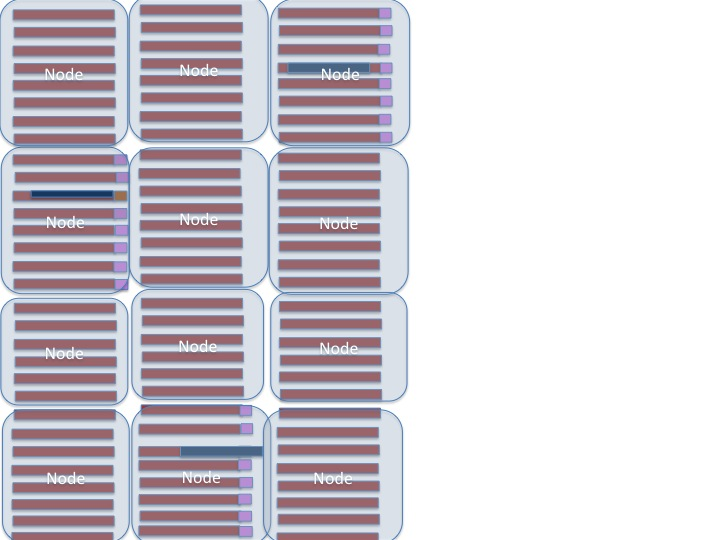
\includegraphics[height=1.3in]{./pictures/NoiseMitigated}}\caption{\label{fig:NoiseTransImbPic}
%      Application timeline schematics.}}
%    \end{figure}
\end{frame}


\begin{frame}[label=mitigationWithinNode]
\frametitle{Within-node Persistent Load Imbalance and Mitigation}
\begin{figure}[ht!]
\label{fig:AppPersistentImbPic}
\subfloat[\tiny Application
  imbalances.]{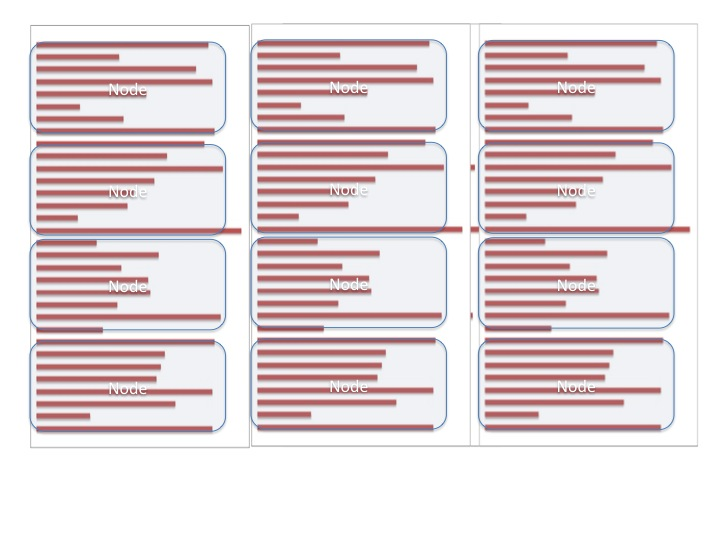
\includegraphics[height=1.3in]{./pictures/PersistentImb2}}\label{fig:AmplificationPic3}\hspace*{0.25in}\subfloat[\label{fig:AmplificationPic3}\tiny
  Mitigated by within-node
  re-distribution.]{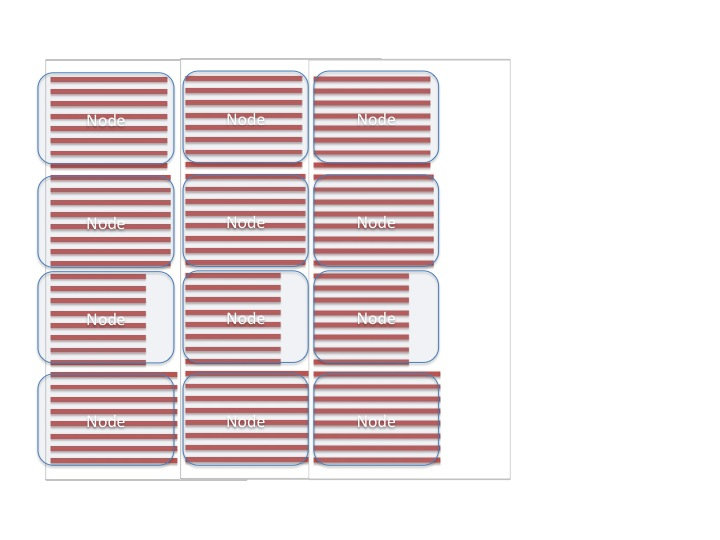
\includegraphics[height=1.3in]{./pictures/PersistentOptimized}}
%\caption{\label{fig:AppPersistentImbPic} Application-induced load
%imbalances.}                                      
\end{figure}
{\small Indent due to not doing across-node balancing, but still much
  better than before.}
\end{frame}

}

%TODO: see if we can change title                           
\comments{ 
\begin{frame}[label=dynLoadBal]
\frametitle{$\rightarrow$ Can Dynamic Load Balancing Fix This?}
\begin{itemize}
\item \small Dynamic load balancing within a node has potential to mitigate imbalances, {\it if} it can be done efficiently.
%\item Dynamic                                              

\begin{itemize}
%\item For both kinds of imbalances.                      
\item \small Persistent imbalance can also be addressed by across-node load balancing (available in Charm++, Zoltan), but it requires more complex machinery (and is complementary anyway).\\
%know questions here 
\end{itemize}
\item \small OpenMP supports dynamic balancing.
\item \small Use OpenMP within-node.
%\begin{itemize}              
%\item \small Is this efficient enough?
%\end{itemize}                                 
\vspace*{.5in}
%\item However, within-node dynamic load balancing faces many                                                     
%challenges.                                        
\end{itemize}
\end{frame}


\begin{frame}[label=hybridstatdyn]
 \frametitle{Hybrid Static/Dynamic Scheduling}
\begin{columns}
  \column{0.5\columnwidth}
  \vspace*{-0.2in}
  \lstinputlisting{./listings/threadedCompRegion-static.c}
  \column{0.5\columnwidth}
%  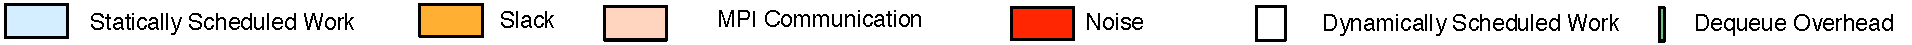
\includegraphics[scale=0.15]{./images/legend-dynamic}\\                                                              
  \vspace*{-0.2in}
  \begin{center}
    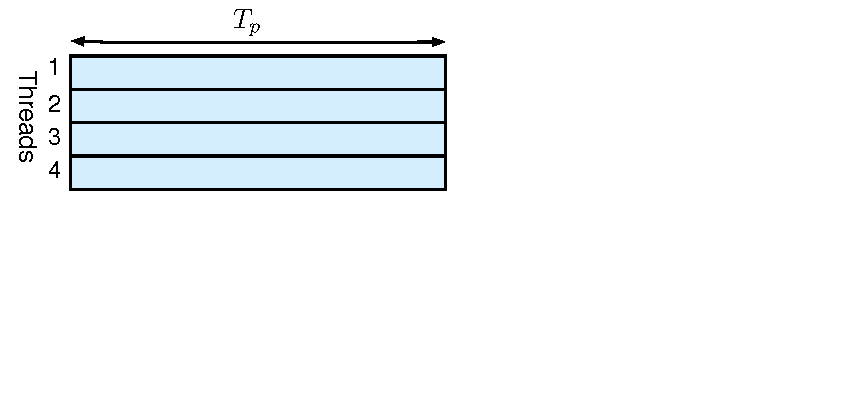
\includegraphics[scale=0.31]{./images/threadedCompRegion-static}
  \end{center}
  \vspace*{-0.4in}
  \begin{center}
    \tiny Susceptible to imbalance.
  \end{center}
\end{columns}
\begin{columns}
\column{0.5\columnwidth}
\vspace*{-0.15in}
\lstinputlisting{./listings/threadedCompRegion-dynamic.c}
\column{0.5\columnwidth}
  \begin{center}
    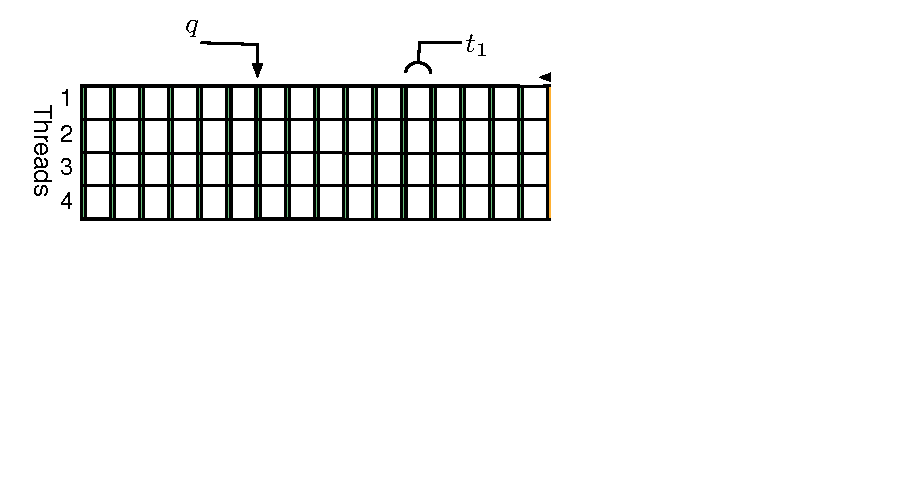
\includegraphics[scale=0.31]{./images/threadedCompRegion-dynamic}
  \end{center}
\vspace*{-0.3in}
\begin{center}
{\tiny Scheduler overhead stretches time.}
\end{center}
\end{columns}
\begin{columns}
\column{0.5\columnwidth}
%TODO: fix code  to be hybrid sched
\vspace*{-0.1in}
\lstinputlisting{./listings/threadedCompRegion-hybrid.c}
\column{0.5\columnwidth}
\begin{center}
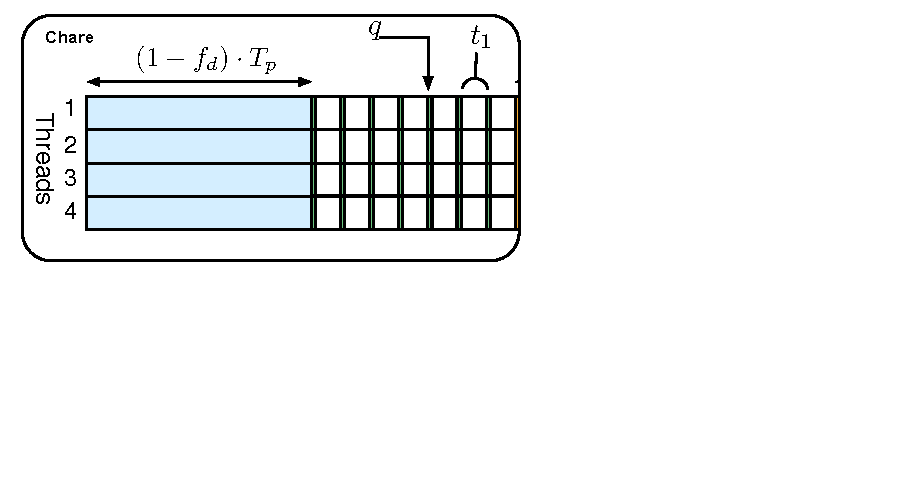
\includegraphics[scale=0.31]{./images/threadedCompRegion-hybrid}
\end{center}
\vspace*{-0.3in}
\begin{center}
{\tiny Can reduce imbalance and sched
  ovhd. simultaneously.\comments{through
    \hyperlink{expTunedSF}{tuning} static fraction.}}
\end{center}
\end{columns}
\end{frame}
}

\begin{frame}[label=halftimings]
\frametitle{Performance with~\hyperlink{expTunedSF}{Tuned} Static Fraction}
\begin{figure}[ht!]
\begin{center}
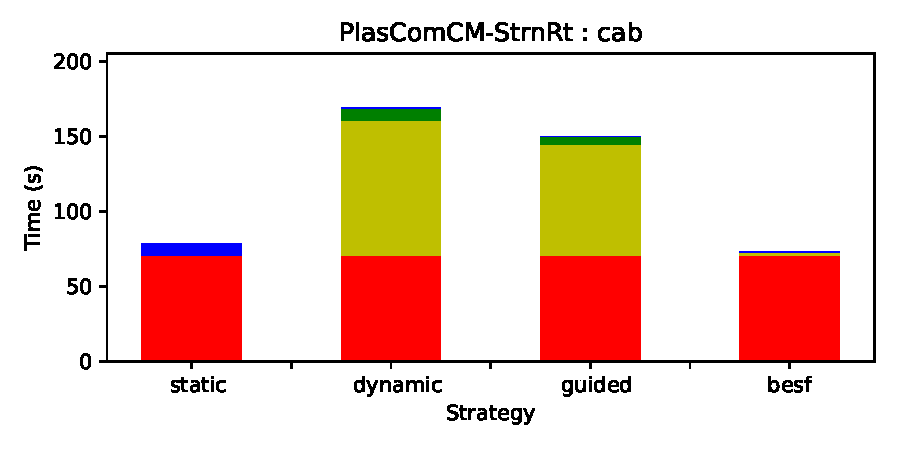
\includegraphics[scale=0.34]{./plots/dmTime-PlasComCM-StrnRt-cab-withbesf}
%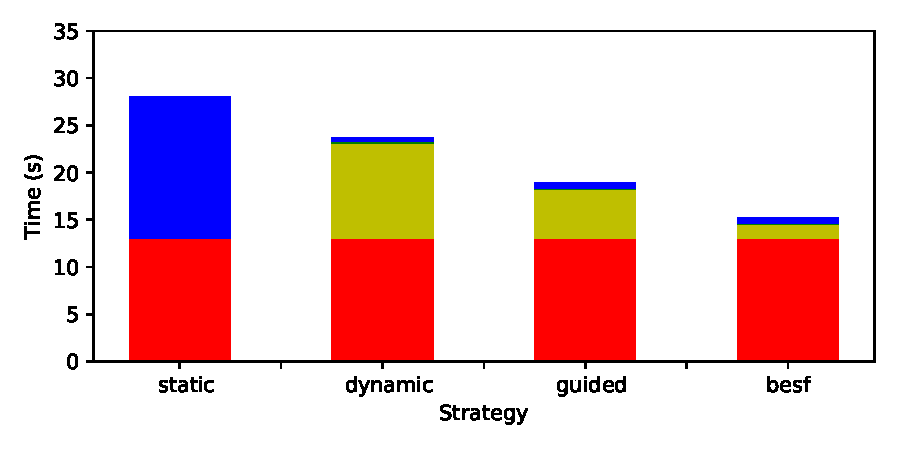
\includegraphics[scale=0.34]{./plots/dmTime-nbody-cab-withbesf}\\
\end{center}
\label{fig:dmTimes-NASLU-cab}
\end{figure}
\begin{center}
{\small In \textit{besf}, we use the best static fraction. See rightmost bar.}
\end{center}
%TODO: fix this so it doesn't duplicate                     
\visible<1->{
\begin{enumerate}
\small \item \small Balances the tradeoff between load balance and
locality
 across applications and platforms. \comments{ Half is better than
   dynamic strategies.  }
\item \small \comments{Even for NASLU,} The \textit{besf} strategy gives performance gains
  over \textit{static}, i.e., the code benefits from the small amount of
  dynamic load balancing.
%\item \tiny Minimizes the costs in each of the three challenges,                                               
%simultaneously.                         
\item \small EuroMPI 2010 : V. Kale and W. Gropp [statdyn] studies
  this idea in more depth.
\end{enumerate}}
\end{frame}

\begin{frame}
\frametitle{PlasComCM Suitability for GPU} 
\begin{itemize} 
\small \item \small PlasComCM has a large number of floating point
operations per grid point per timestep \comments{ $\rightarrow$ easy to vectorize}
\item \small These computations are repeated over
  timesteps \comments{$\rightarrow$ ease of programmability}. 
\end{itemize} 
{\small Can an accelerator architecture provide significant performance
benefit for stencil-type computation on structured grids?} 
\end{frame} 

\begin{frame}[label=perfExp]
\frametitle{Performance Expectation Using GPU} 
\begin{itemize} 
\small \item \small Efficient assuming all data can fit in memory. 
%\item \small How many GPUs needed to fit application data? 
\item \small Consider just the 2D axi-symmetric problem. 
\item \small We only need 1 (allowing data to be held in GPU memory). 
\item \small Future archs may have \texttt{nvlink}, other technology.  
\end{itemize} 
% Be optimistic and theorize. 
\end{frame} 

\comments{
\begin{frame}[label=cid] 
\frametitle{3D 7-point Stencil Results} 
\begin{center} 
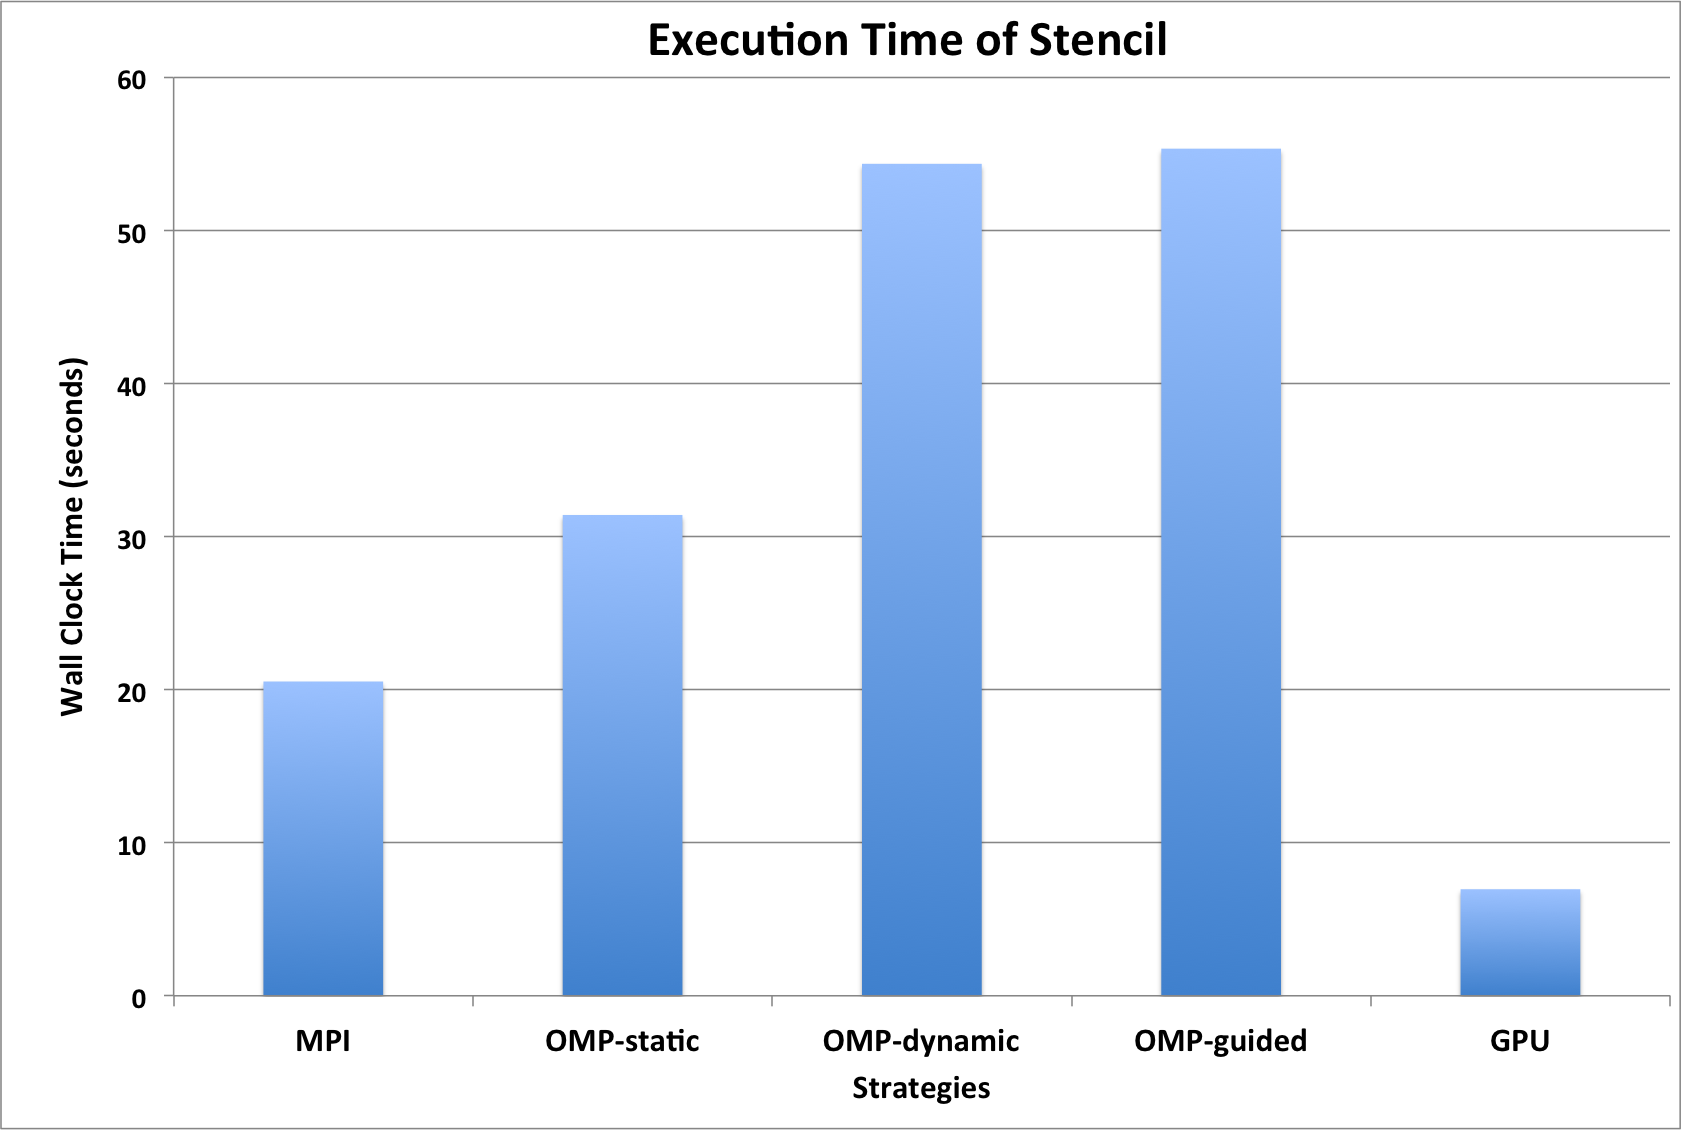
\includegraphics[scale=0.24]{./plots/stencilGPUresults} 
\end{center} 
\end{frame} 


\begin{frame}[label=cid]
\frametitle{PlasComCM Results/Projections for CID} 
\begin{center}
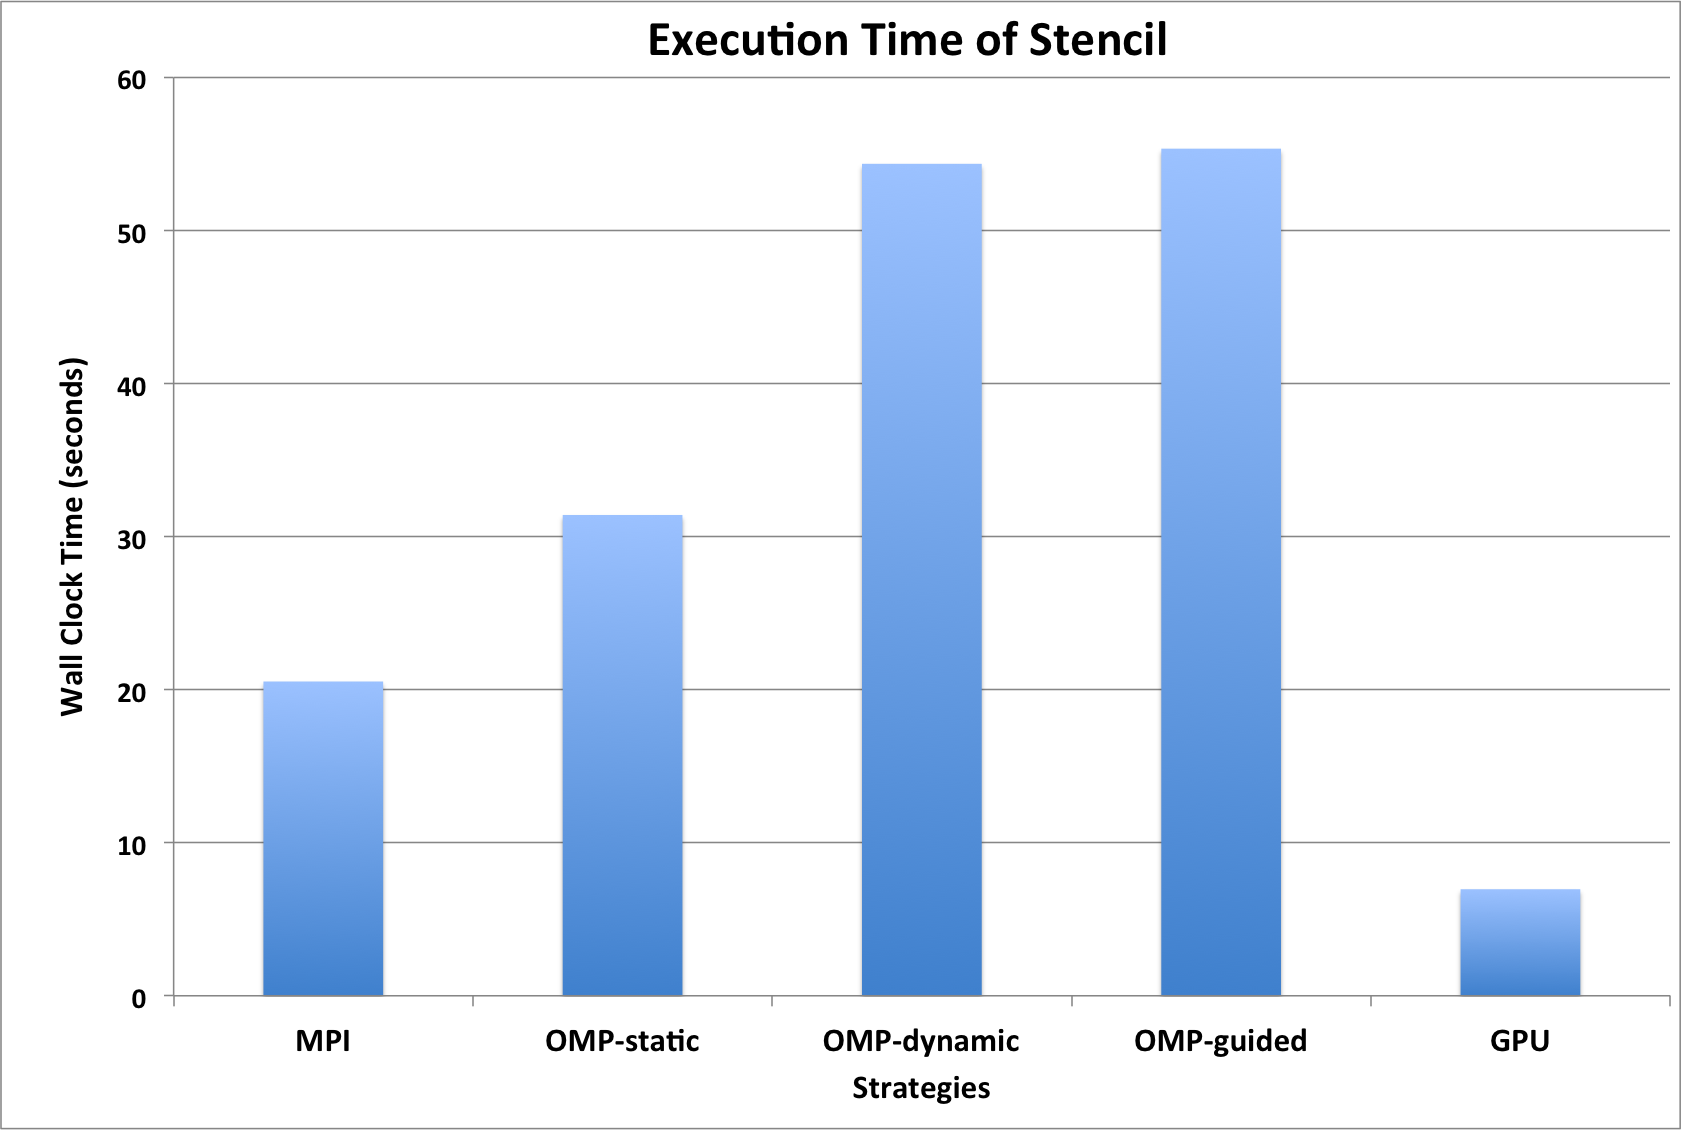
\includegraphics[scale=0.18]{./plots/stencilGPUresults} \hspace*{0.2in} 
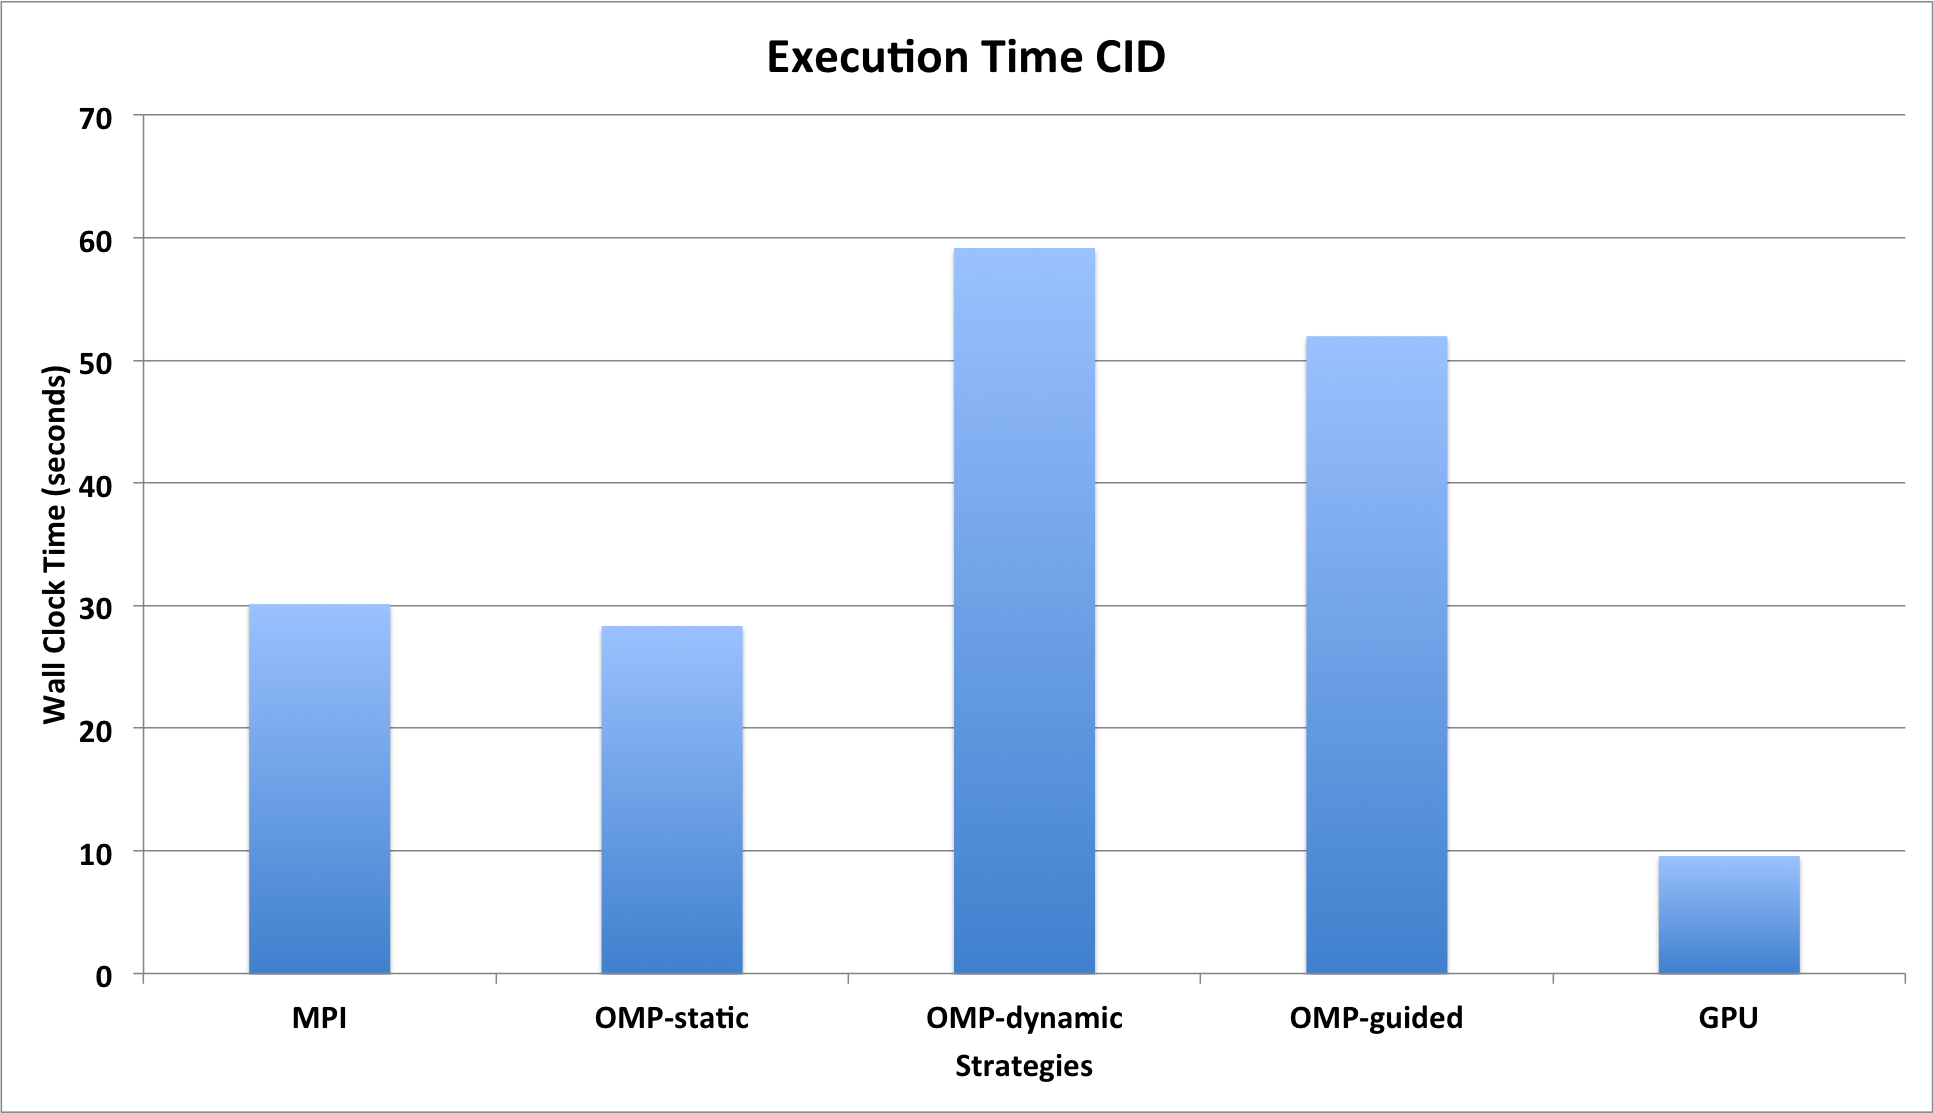
\includegraphics[scale=0.18]{./plots/CIDGPUresults} 
\end{center} 
\end{frame}}  

\comments{
\begin{frame} 
\frametitle{Timing the Functions}  

Used pgcc compiler
\end{frame}
}

\begin{frame}[label=strnrt]
\frametitle{PlasComCM Results/Projections for StrnRt} 

\begin{itemize} 
\tiny \item \tiny Ran PlasComCM code with 2D axi-symmetric problem as input on one node of the xpacc
cluster. 
\item \tiny One MPI process / OpenMP thread per core used for CPU
version. 
\item \tiny Timing done for the StrnRt function only. 
\end{itemize} 

\begin{center} 
% 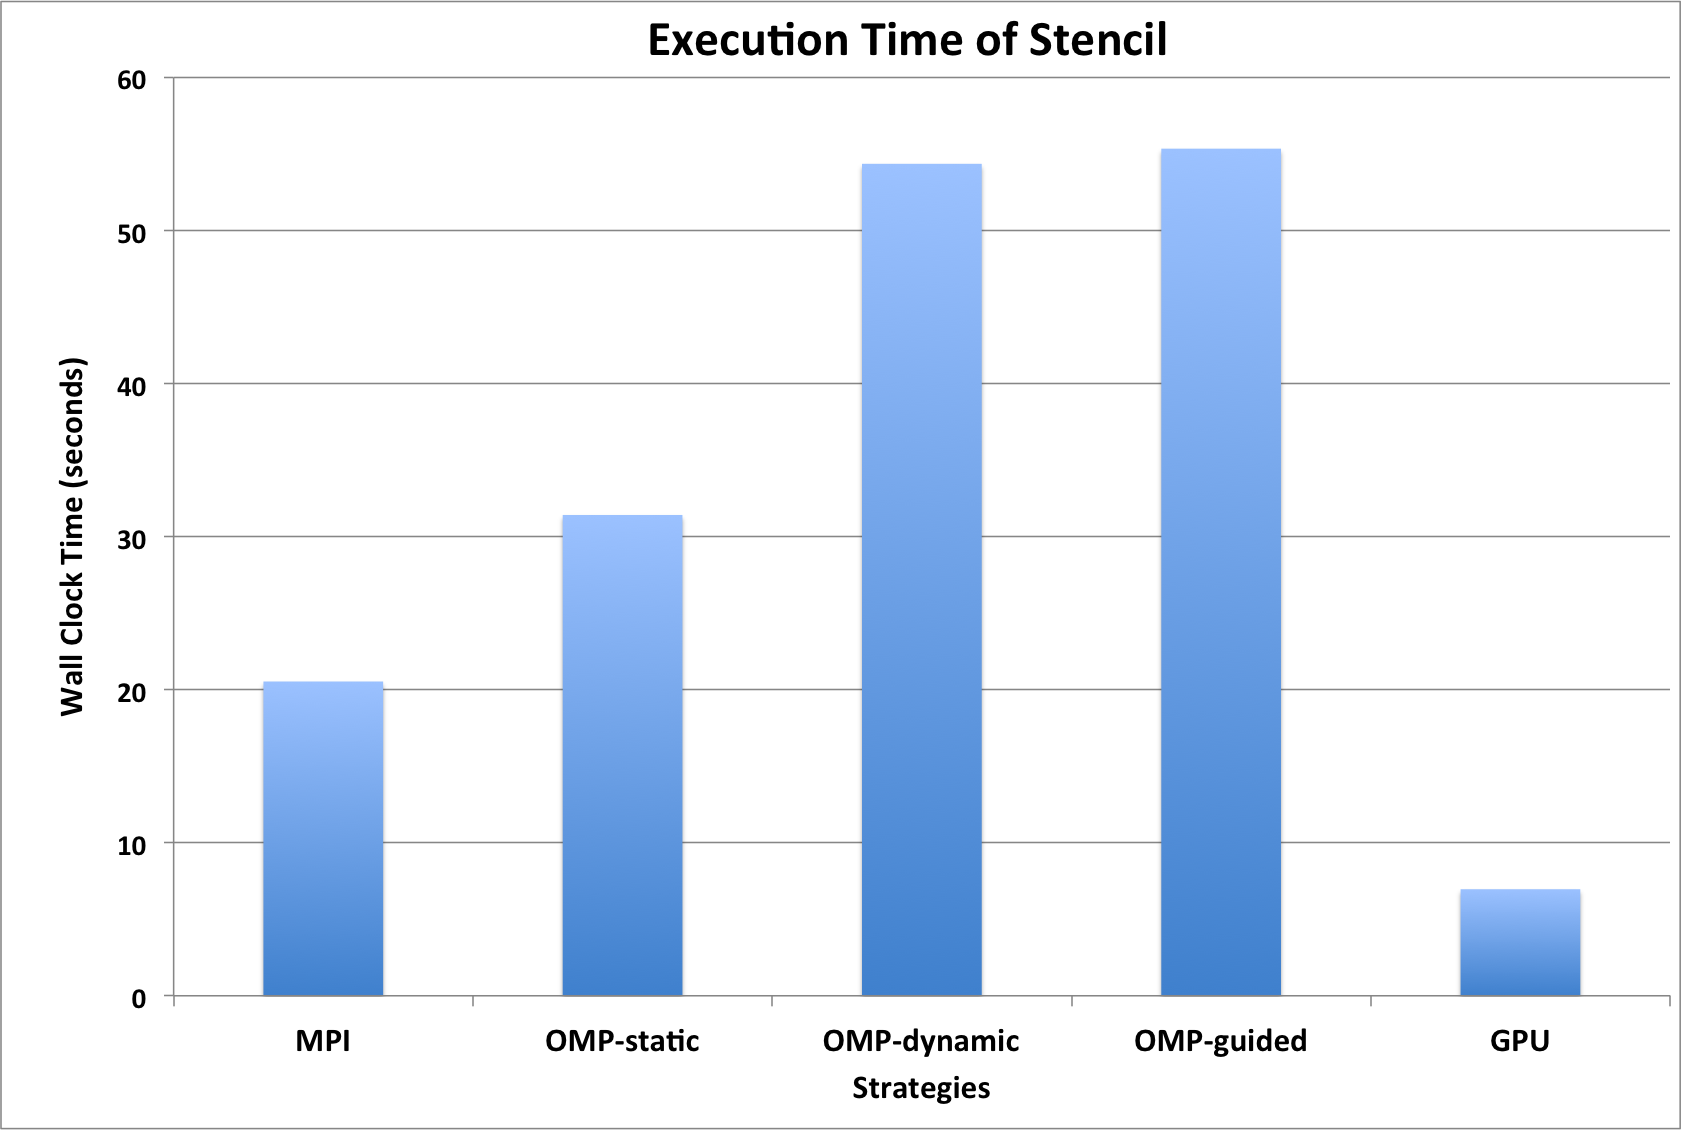
\includegraphics[scale=0.18]{./plots/stencilGPUresults} \hspace*{0.2in} 
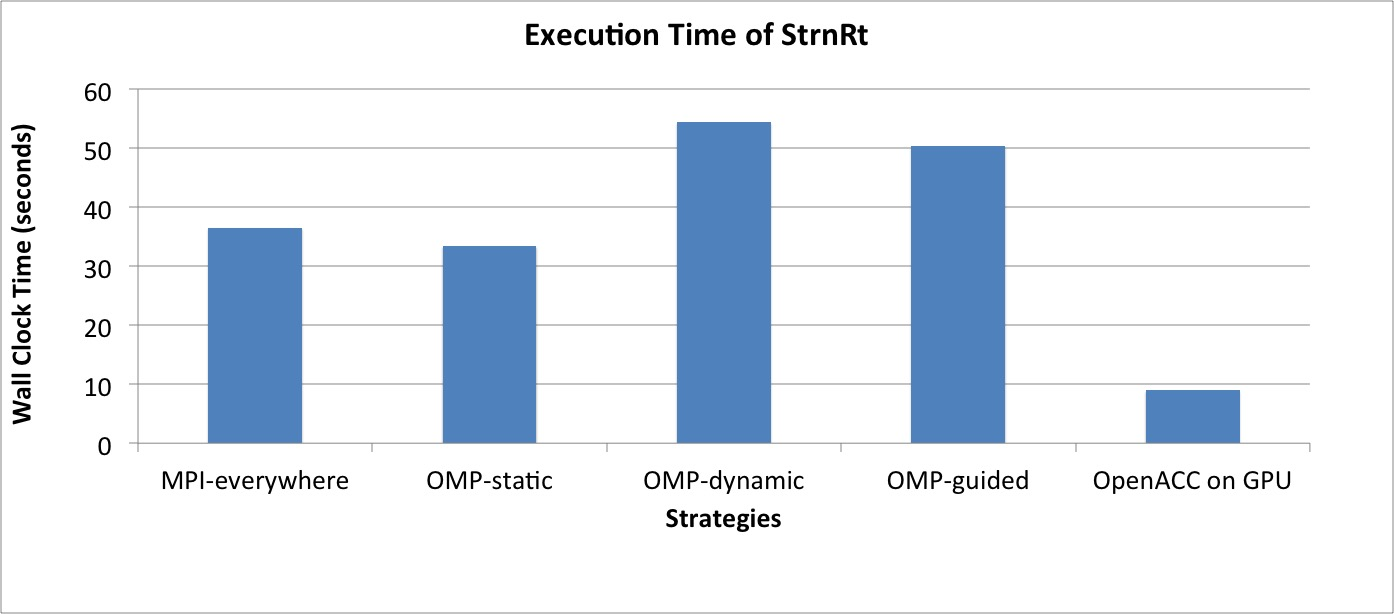
\includegraphics[scale=0.22]{./plots/StrnRtGPUresults} 
\end{center}

\begin{enumerate} 
\tiny \item \tiny OpenMP version with static scheduling run on CPU degrades performance. 
\item \tiny MPI version run on CPU gets 3x performance improvement
  over OpenACC version on GPU. 
\end{enumerate} 
\end{frame} 
\comments{
\begin{frame} 
  \frametitle{How it Fits in the Bigger Picture}
\end{frame} 
}

\begin{frame}[label=impqual]
\frametitle{Questions that follow: Implementation Quality} 
\begin{columns} 
\column{0.5\columnwidth}
\underline{\textbf{CPU }}
\begin{itemize} 
\small \item \small memory bandwidth limitation $\rightarrow$ measure
off-chip cache misses.
\item \small performance variations $\rightarrow$ calculate idle time 
\item \small Others?
\end{itemize}

\column{0.5\columnwidth}
\underline{\textbf{GPU } } 
\begin{itemize} 
\small \item \small Vectorization of code $\rightarrow$ compiler's vectorization report.
\item \small Efficient of use of GPU cores i.e.,  $\rightarrow$ calculate floating point intensity 
\item \small Others? 
\end{itemize} 
\end{columns} 
\end{frame} 

\begin{frame}[label=relatedWork]
\frametitle{Related Work} 
\begin{itemize} 
%\small \item \small PlasComCM paper

\small \item \small Exploring Programming Multi-GPUs Using OpenMP and OpenACC-Based Hybrid Model. Rengan Xu, Sunita Chandrasekaran, Barbara Chapman. 
\item \small Hyesoon Kim, Richard Vuduc, Sara Baghsorkhi, Jee Choi,
  and Wen mei Hwu. Performance analysis and tuning for general purpose graphics processing units (GPGPU). Synthesis Lectures on Computer Architecture. Morgan \& Claypool Publishers, San Rafael, CA, USA, November 2012.
%\item \small GPU paper
%Work-stealing/Cilk: Leiserson and group at MIT 
%Schedule all events together to make only
%  some timesteps be impacted by noise, but can't co-schedule all events.
\end{itemize}
\end{frame} 

%\small \item \small Original MPI code run on CPU with 16 cores: 34.45 ms
%\item \small Transformed OpenACC code run on GPU: 8.34 ms 

\begin{frame} 
\frametitle{Conclusions}
\begin{enumerate} 
  \small \item \small Need low-overhead scheduling strategies for
      improving performance of scientific applications.
    \item \small Many different factors when running an application on a particular architecture. These require multiple low-overhead scheduling strategies to be used at once.
%    \item \small Results show that composition is additive in
%      performance.
   \item \small Future work: (a) Integration with OpenMP or other
      shared memory model; (b) composition with other scheduling
      strategies (which includes generalized methodology for composition for future scheduling strategies). 
%\small \item \small Using GPU can be beneficial for PlasCom over MPI version, if not for
%  current machines, then for future machines. 
\item \small Using OpenACC-ized version of PlasComCM on GPU could be
beneficial over MPI version of PlasComCM on CPU. 
\small \item \small Using OpenACC-ized version of PlasComCM on GPU is
also likely beneficial over OpenMP-ized version of PlasComCM on CPU. 
\item \small Current results will be extended upon to show feasibility. 
\end{enumerate} 
\end{frame} 


\begin{frame}[label=ack] 
  \frametitle{Acknowledgements}
  \begin{itemize}
  \item John Larson - performance models and implementation discussion
%  \item Simon Garcia - discussion of OpenCL code
  \item Jon Freund - Guidance for overall project
  \item Luke Olson - Discussion of input problem sizes
  \item Micheal Klemm - Discussion of OpenACC
  \item Dan Bodony -  Ongoing discussion of PlasComCM data partitioning
%  \item Todd Gamblin: Software
%    \item Franck Cappello: Noise modeling based on fault-tolerance models  
%    \item Torsten Hoefler: amplification and slack description 
%    \item Laura Grigori: CALU scheduling 
%    \item Micheal T. Heath: Suggestions on theoretical analysis and
%      formalization of performance models. 
  \end{itemize}
\end{frame} 

\comments{
\begin{frame}[plain,c]
  \begin{center}
      Appendix
  \end{center}
\end{frame} 
}

\comments{
\begin{frame}[label=mitigationWithinNode]
\frametitle{Within-node Persistent Load Imbalance and Mitigation}
\begin{figure}[ht!]
\label{fig:AppPersistentImbPic}
\subfloat[\tiny Application
  imbalances.]{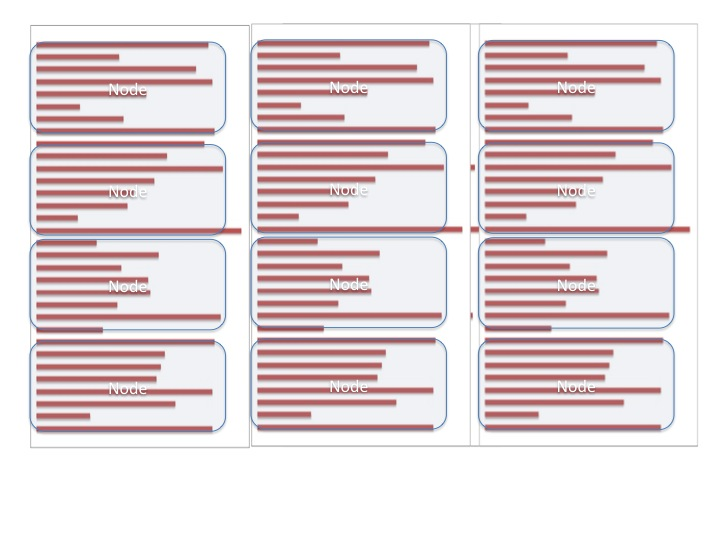
\includegraphics[height=1.3in]{./pictures/PersistentImb2}}\label{fig:AmplificationPic3}\hspace*{0.25in}\subfloat[\label{fig:AmplificationPic3}\tiny
  Mitigated by within-node
  re-distribution.]{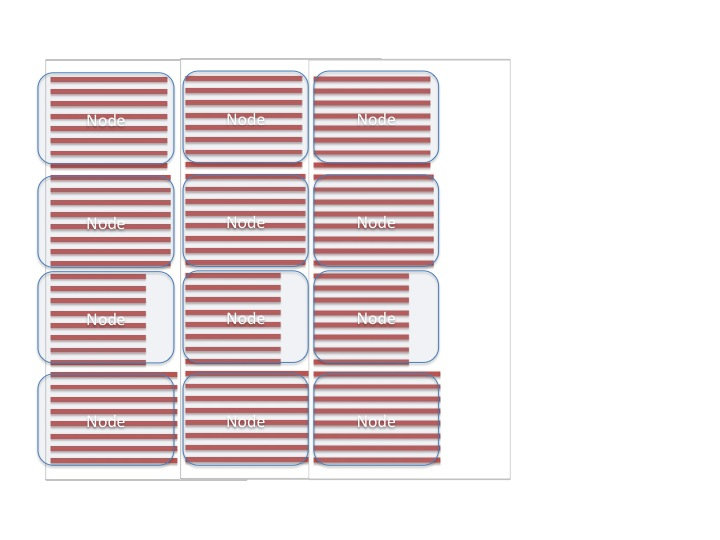
\includegraphics[height=1.3in]{./pictures/PersistentOptimized}}
%\caption{\label{fig:AppPersistentImbPic} Application-induced load
%imbalances.}                                      
\end{figure}
{\small Indent due to not doing across-node balancing, but still much better than before.}
\end{frame}
}

\comments{}  

%\begin{frame}{Results with PlasComCM}
%\todo{VK: Add results to this slide.} 
%\end{frame}


\begin{frame}{Work on Application Code for X-ray Imaging at USC/ISI} 
\begin{enumerate} 
\item Performance assessment 
\begin{itemize} 
\small \item \small Computational requirements to calculate number of GPUs needed. 
\item \small Ensured that a dedicated network, similar to ESnet, doesn’t slow down computation: our application has unique requirements in that we need to stream the input data from data source to the supercomputer center.
\end{itemize}
\item Performance optimization.
\begin{itemize} 
\small \item \small Ptychography code optimization: compiler flag optimization, loop unrolling, started work on half-precision instructions for NVIDIA Tesla P100.
\item \small Tomography code optimization: discussed and worked on translating matlab code to C++ code, including working on numerical optimization.
\end{itemize}
\item Procurement of resources to set up experiments.
\begin{itemize}
\small \item \small Obtained machine resources from University of Southern California's High Performance Computing Center.
\small \item \small Worked on proposal for Intel MICs to add to USC HPC system.
\end{itemize}
\end{enumerate}
\end{frame} 

\begin{frame}{What We Are Trying To Do}
\begin{enumerate} 
\item Overview of problem/solution: Image reconstruction of 3-d chip : explain problem from Broad Agency Announcement. 
\item Implementation details of problem/solution: Figure of overall problem: 
\item Coherent Diffraction Imagery:  
\begin{itemize} 
\small \item \small 2-dimensional Reconstruction:  ptychography 
\item \small 3-dimensional reconstruction from slices generated by ptychography using tomography algorithms. 
\end{itemize} 
\end{enumerate}
\begin{figure}[ht!]
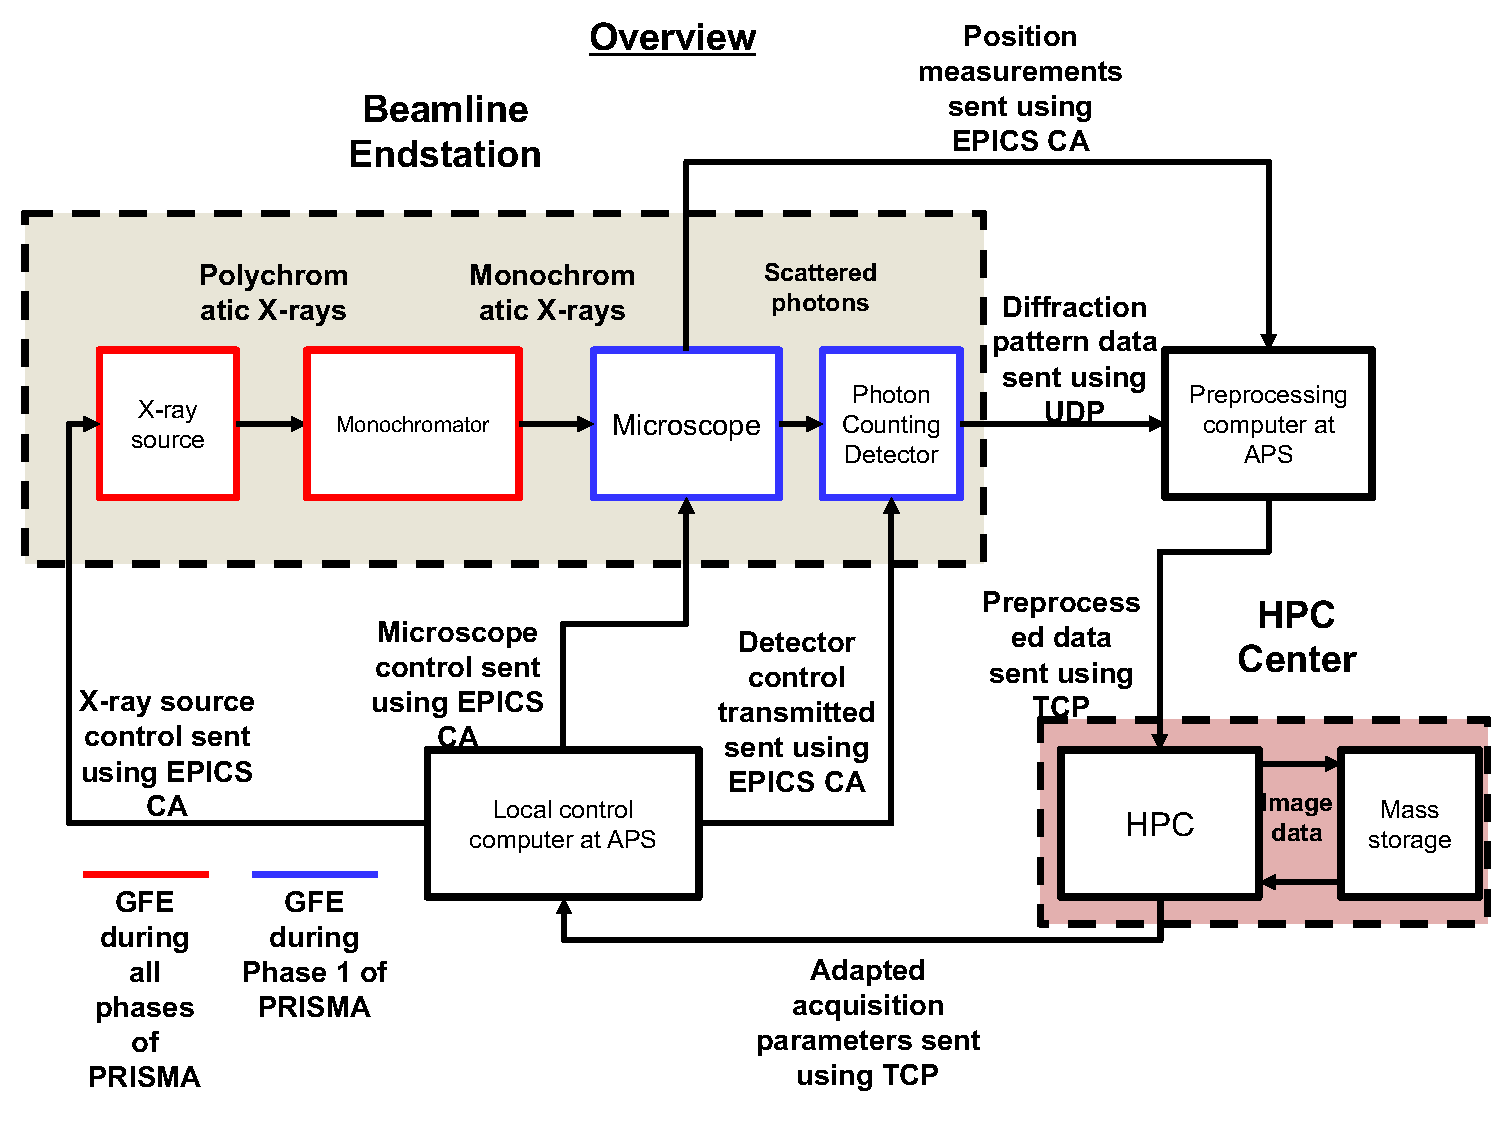
\includegraphics[scale=0.22]{./images/exp_schematic_1017_1}
\end{figure} 
\end{frame}

\begin{frame}{Computational Aspects of Problem} 
\begin{figure}[ht!]
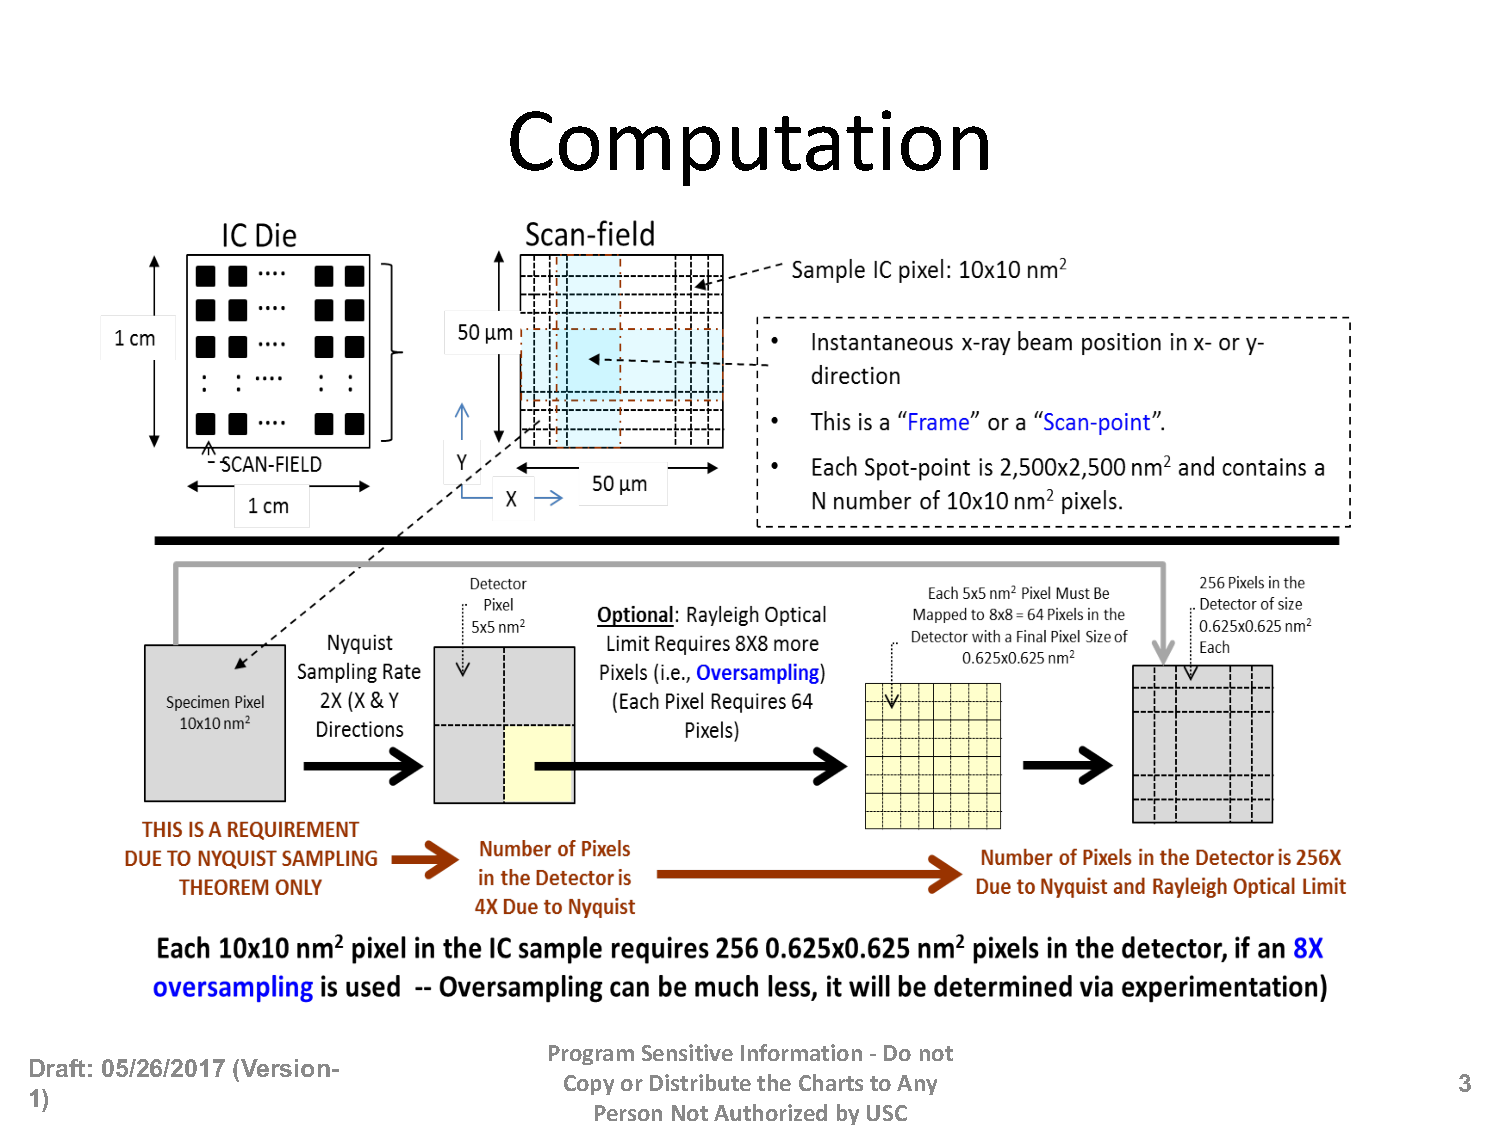
\includegraphics[scale=0.4]{./images/exp_schematic_1017_2}
\end{figure}
\end{frame}

\begin{frame}[label=AppUnderstanding]
\frametitle{Understanding Numerical Algorithm}
{\small \underline{\bf X-ray Imaging Algorithms}}
\begin{itemize}
\tiny \item \tiny Use ePIE due to memory footprint of DM. DM uses 5 GB because it stores buffers for current and previous wavefront while ePIE uses 1 GB.
\tiny \item \tiny ePIE tries to recover two distinct quantities: (1)
the probe wavefront describing the beam incident on a sample and (2) the object transmission function describing the sample under
investigation.
\end{itemize}
{\small \underline{\bf Code}}
\begin{itemize}
\item \tiny ePIE is embarassingly parallel with collective communication at the end.
\item \tiny Updates the object and probe function on each iteration.
\item \tiny Steps to update the object and probe function are repeated for every diffraction pattern j and for a number of ePIE iterations, or until a certain convergence criterion is met.*
\end{itemize}
{\small \underline{\bf Performance Optimizations}}
\begin{itemize}
\tiny \item \tiny Uses NVIDIA cuFFT library for optimization of FFT calculations.
\item \tiny Uses DIY library for partitioning of data across nodes.
\item \tiny Uses memory coalescing on GPU and partitioning of data onto GPU for load balancing.
\end{itemize}
{\tiny \textit{Parallel Ptychographic Reconstruction. Nashed et al.}}
\end{frame}

\begin{frame}{Procurement of Resources to Set Up Experiments} 
\begin{enumerate} 
\item Obtained GPU machine resources from USC HPC
\begin{itemize}
\small \item \small Focused on applications for ptychography, which is
a compute-intensive code with same work repeated across outer loop
iterations. 
\small \item \small Benchmarking. 
\end{itemize}
\item Worked on proposal for Intel MICs to add to USC HPC system.
\begin{itemize} 
  \small \item \small Justified adding Intel Xeon Phi to existing HPC
  system to run experiments of OpenMP-ized version of the code. 
\end{itemize} 
\item Worked on network infrastructure. 
\begin{itemize} 
\item \small benchmarking to know existing capabilities.
\item \small Burst buffers. 
\item \small Provisioning. 
\end{itemize}
\end{enumerate}
\end{frame} 

\begin{frame}{Performance Assessment}
\begin{enumerate}
\item Performance Profiling
\begin{itemize}
\item Used CUDA PAPI to profile cache misses of MPI+CUDA, leads to work on roofline model.
\item Looked into call-path + causal profiling for MPI+CUDA for identifying where FFTs are called. 
\item Looked at tomography code performance to project number of GPUs needed. 
\end{itemize} 
\item Performance Modeling
\begin{itemize}
\item Computational requirements to calculate number of GPUs needed. 
\item Ensured that a dedicated network, similar to ESnet, doesn’t slow down computation: our application has unique requirements in that we 
  need to stream the input data from data source to the supercomputer center. 
\end{itemize} 
\end{enumerate} 
\end{frame} 

\begin{frame}[label=scalingptycho]{Performance Modeling of Computation}
\begin{itemize}
\tiny \item \tiny 
\item \tiny 
\end{itemize} 
\begin{figure}[ht!]
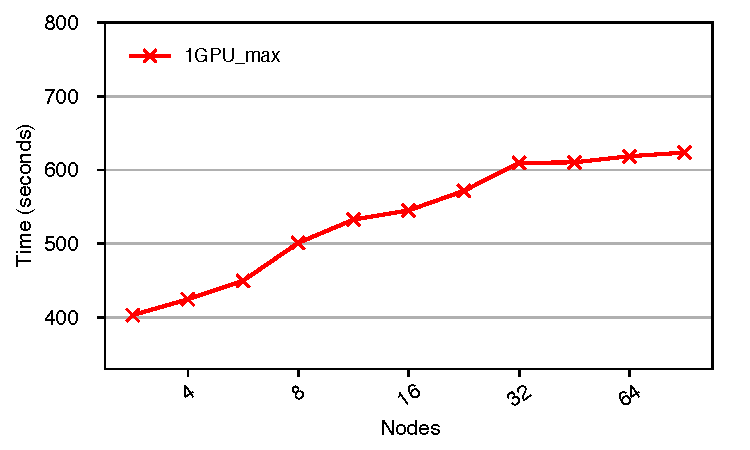
\includegraphics[scale=0.5]{./plots/ptychoLib-hpcc-weakscale-intro.pdf}
\end{figure}
\underline{\bf Timings for Tomography:} 1 CPU with full problem size:
20 seconds, 1 MPI process '' '': 12.0 seconds , 16 MPI processes: 2.75 seconds 
\underline{\bf Timings for Tomography(weak Scale):} 32 MPI processes
on two nodes: 3.34 seconds | 64 MPI processes on 4 nodes: 4.10 seconds 

%\begin{figure}[ht!]
%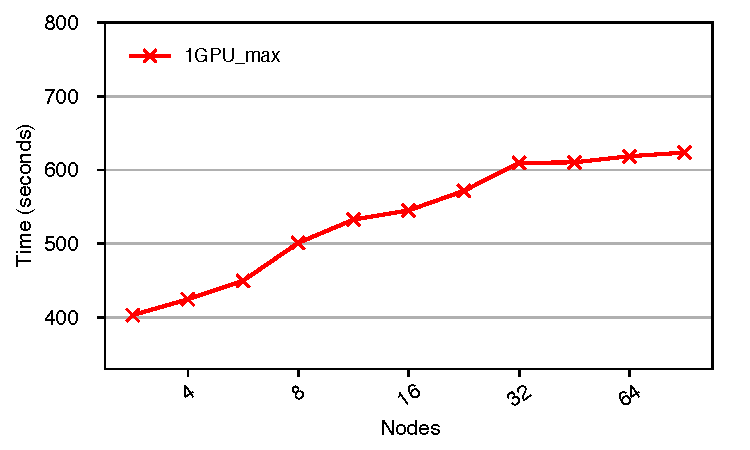
\includegraphics[scale=0.5]{./plots/ptychoLib-hpcc-weakscale-intro.pdf} 
%\end{figure} 
\begin{enumerate}
\tiny \item \tiny 
\item \tiny 
\end{enumerate}
\end{frame}


\comments{ 
\begin{frame}[label=mpicudaprofile]{MPI+CUDA Call-path and Causal Profiling}
\end{frame}

\begin{frame}[label=mpicudaprofile]{MPI+OpenACC NAS Benchmarks}
\end{frame} 

}


\begin{frame}{Performance Optimizations}{} 
\begin{enumerate}
\item Ptychography code optimization.
\begin{itemize}
\small \item \small compiler flag optimization.
\item \small loop unrolling. 
\item \small started work on half-precision instructions for NVIDIA Tesla P100. 
\end{itemize}
\item Tomography code optimization. 
\begin{itemize} 
\small \item \small discussed and worked on translating matlab code to C++ code.
\item \small including working on numerical optimization.
\end{itemize}
\item Input data transfers. 
\begin{itemize} 
\small \item \small Compression of data. 
\item \small Middleware for data storage, e.g., HDF5 .  
\end{itemize} 
\end{enumerate} 
\end{frame}


\comments{
\begin{frame}{Performance Optimization of Ptychography Code}{Using Half-precision Instructions} 
%\begin{lstlisting}
%\lstinputlisting{./listings/halfPrecisionCodeSnippet.cc}
%\end{lstlisting}
\end{frame}

\begin{frame}{Performance Optimization of Ptychography Code}{Compiler Optimizations and Loop Unrolling} 
\end{frame} 
}

\begin{frame}{Results of Performance Optimization of Ptychography Code}
\begin{itemize}
\item Using loop transformations on a variety of compiler flag optimizations on the ptychoLib code improves performance of the
ptychoLib code by 12.2\%. 
\item Using Tesla P100 half-precision instructions on code
  representative of PtychoLib improves performance of the code by
  13.2\% (--TODO: check this through back-of-envelope calcs--)
\end{itemize}
\end{frame}

\comments{
\begin{frame}{Performance Optimization of Tomography Code}{Using MPI C++ instead of MATLAB}
\begin{figure}
    \centering
 \lstinputlisting{./listings/tomographyCode.cc}
    \caption{Code for Tomography}
    \label{fig:my_label}
\end{figure}
\end{frame} 

\begin{frame}{Performance Optimization of Tomography Code}{Numerical Algorithm and Memory Optimization}
\begin{figure}
    \centering
\lstinputlisting{./listings/tomographyCode2.cc}

    \caption{}
    \label{fig:my_label}
\end{figure}
\end{frame} 

\begin{frame}{Results of Performance Optimization for Tomography Code}
  \begin{itemize}
    \tiny \item \tiny  Average of 1.49 seconds. Std deviation: 0.02 seconds. Over 5 trials.
  \end{itemize}
\end{frame} 

}


\comments{
\begin{frame}[label=proposalTimeAlloc]
\frametitle{Proposal for Parallel Machine Time Allocation}
%Application for access to USC compute resources.% 

\begin{outline}[enumerate]
\tiny \1 {\tiny Context and Goal}
\tiny \2 {\tiny Context: need to better understand behavior of
  Integrated Circuits(IC)/computer chips technology to make
  advancements IC technology.}
\tiny \2 {\tiny Goal: Construct an image to simulate operation of
  integrated circuit.}
\tiny \3 {\tiny The following requirements for image reconstruction
are needed: Real-time feedback during imaging, use of x-ray sources,
establish highly reliable program.}
\tiny \1 {\tiny Project Methodology: How will you proceed? What kind
of data or software will you use or install?}
\tiny \2 {\tiny Use Ptychography technique to generate a 2D image and
  then use tomography to combine the 2D images to 3D images.}
\tiny \2 {\tiny Data and Software:}
\tiny \3 {\tiny software: Ptycholib for constructing ptycholib algorithms.}
\tiny \3 {\tiny For data for doing experimentation, we'll use Argonne's advanced photon source.}
\tiny \1 {\tiny Justification: (How will HPC use improve your results and help acheive your goals)}
\tiny \2 {\tiny Ptychography is computationally intensive with FFTs. }
\tiny \2 {\tiny GPU resources allow for throughput computing and will
  help improve efficiency of our simulations.}
\tiny \2 {\tiny interconnect network of cluster will help to improve efficiency of FFT algorithms.}
\2 {\tiny The improvements in efficency can help with doing more
scientific calculations per second so as to allow for achieving high
resolution images and satisfying the three requirements described in
the response of the prompt Project Methology.} 
\end{outline}

\end{frame}  

}

\begin{frame}{Dynamic Scheduling for Communication-avoiding Dense Matrix Factorization}{Overview}
\begin{itemize}
\item Locality-Aware Scheduling for CALU/CAQR: Performance Variability Results and Software Development.
\item Low-overhead Loop Scheduling for CALU/CAQR: Performance Variability Results and Theoretical Analysis.
\end{itemize}
\end{frame}


\begin{frame}[label=dynworkovw]{Dynamic Loop Scheduling in OpenMP}{An Overview}
\begin{enumerate}
\item User-defined Loop Scheduling
\begin{itemize}
\item Allows users to define their own loop schedules, in particular those with data locality.
\end{itemize}
\item Locality-Aware Task Scheduling: Supporting Locality for Tasking.
\begin{itemize}
\item \small Working with Martin Kong from Brookhaven National Laboratory.
\item \small Based on work of Vivek Sarkar.
\end{itemize}
\end{enumerate}
\end{frame}

\begin{frame}{OpenMP Loops Redux}
OpenMP provides a loop worksharing construct that specifies: 
\begin{itemize}
\item How the logical iteration space of a loop is cut into chunks
\item How the resulting chunks are assigned to the work threads of the parallel region.
\end{itemize}
  
%\begin{verbatim}
% # pragma omp for \[clause\[ \[,\] clause\] ... \]
%      for (int i=0; i<100; i++){}
%\end{verbatim}

\begin{itemize}
\item Loop needs to be in canonical form, that is, adhere to certain properties
\item The clause can be one or more of the following: \texttt{private(...)}, \texttt{firstprivate(...)}, \texttt{lastprivate(...)}, \texttt{linear(...)}, \texttt{reduction(...)}, \textbf{schedule(...)}, collapse(...), ordered[...], nowait, allocate(...) 
\item We focus on the clause \textbf{schedule()}
\end{itemize}

\end{frame}

\begin{frame}{Need Novel Loop Scheduling Techniques in OpenMP}

\begin{enumerate}
\item Supercomputer architectures and applications are changing.
\begin{itemize}
\small \item \small Large number of cores per node.
\item \small Speed variability across cores.
\item \small Complex dynamic behavior in applications themselves.
\end{itemize}
\item So, we need new methods of distributing an application’s parallelized loop's iterations to cores.
\item Such methods need to: 
\begin{itemize}
\small \item \small Ensure data locality, reduce synchronization overhead and maintain load balance~%\cite{worksteal99, dynwork2}.
\item \small Be aware of inter-node parallelism handled by libraries such as MPICH3~%\cite{mpich2}. 
\item \small Be suitable for the needs of a particular loops and machine characteristics.
\item \small Adapt during an application's execution.
\end{itemize}
\item Some customer demand for the SSG-DRD EMEA HPC team.
\end{enumerate}
\end{frame}




\begin{frame}{Utility of Novel Strategies Shown} 
\begin{itemize}
\item Utility of novel strategies is demonstrated in published work by V. Kale et al 1,2 and others.
\item For example, mixed static-dynamic scheduling strategy with an adjustable static fraction.
\item To limit the overhead of dynamic scheduling, while handling imbalances, such as those due to noise.
\end{itemize}
\end{frame}

\begin{frame}{Intel-specific Loop Schedules}
Intel’s (and LLVM's) OpenMP runtime offer additional scheduling types:
\begin{itemize}
\small \item \small E.g., static stealing
\item \small Are accessed through \texttt{schedule(runtime)} and \texttt{OMP\_SCHEDULE} environment variable
\item \small Cumbersome to use; very complex to extend (need to modify the RTL code and recompile the RTL code)
\item \small Not portable across OpenMP implementations
\item \small Proposed user-defined scheduling (UDS) will provide a portable and flexible way of extending OpenMP’s loop scheduling types.
\end{itemize}

\end{frame} 


\begin{frame}{ Specification of a User-defined Scheduling Scheme} 

\begin{enumerate}
\item We aim to specify a user-defined scheduling scheme within the OpenMP specification1 .
\item The scheme should accommodate an arbitrary user-defined scheduler.
\item These are the elements required to define a scheduler.
\begin{itemize}
\item Scheduler-specific data structures.
\item History record: adapt the loop schedule based on previous loop invocations and/or user-specified carry parameters. 
\item Specification of scheduling behavior of threads.
\end{itemize}
\end{enumerate} 
\end{frame}



\begin{frame}{ Proposal for a User-defined Schedule in OpenMP} 
This example gives a glimpse at how a user-defined schedule might look like:


\begin{figure}[ht!]
\lstinputlisting{listings/omp-uds-example.c}
\end{figure}

\begin{itemize} 
\item The \texttt{declare schedule} directive is used to connect a schedule with a set of functions to initialize the schedule and hand out the next chunk of iterations.
\item The syntax of the \texttt{schedule} clause is extended to also accept an identifier of 
\item Instead of calling into the RTL for loop scheduling, the compiler will invoke the functions of the UDS 
\item Visibility and namespaces of these identifiers will be borrowed from UDRs
\end{itemize}  
\end{frame} 
%\begin{frame}{ An Implementation of the Dynamic Schedule with UDS} 
%\end{frame} 
%\begin{frame}{An Implementation of the Static Schedule with UDS}
%\end{frame} 

\begin{frame}{An Implementation of the Static/Dynamic Schedule with UDS}

\begin{figure}
    \centering 
    \lstinputlisting{listings/openmpudsdyndatstruct.c}
    \caption{Caption}
    \label{fig:my_label}
\end{figure}
\end{frame} 

\begin{frame}{Issues to Consider}
\begin{enumerate} 
\item Modifiers to clause: non-monotonic 
\begin{itemize}
\item Problem: How do we handle loop having indices that are non-monotonic?
\item Code example: 
\item Solution: For the proposal, we restrict users to to use monotonic loops for now
\end{itemize}
\item How do schedules guarantee correct execution when a global variables are used?
\begin{itemize}
\item Problem: 
\item Code example: 
\item Solution we propose: 
\end{itemize}

\item Compatibility with clause concurrent: 
\begin{itemize}
\item Problem: See e-mails from Xinmin et al on this, including definition of concurrent in the classical sense.
\item Code example showing problem:
\item Proposed Solution: can enforce that concurrent not be used with user-defined schedule. 
\end{itemize}
\end{enumerate}

\end{frame}


\begin{frame}{Implementation Specifics in LLVM} 

\begin{itemize}
\item Modify in LLVM OpenMP runtime. 
\begin{itemize}
\small \item \small Kmp\_sched.c
\end{itemize}


\item Modify LLVM's OpenMP compiler. 
\begin{itemize}
\small \item \small Would like help from people to do this to get a reference implementation done in a timely manner. 
\end{itemize} 

\end{itemize}

\end{frame}


\begin{frame}{Current Status of the Proposal}{}
\begin{itemize}
\item Vivek Kale (external) presented the proposal at OpenMPCon and IWOMP
\item There is a scientific paper showing the merits of UDS in general (using a prototype implementation based on macros)
\item A report out of Vivek and myself has been scheduled for the FTF in Austin in ww05
\item We are working on the syntax details plus a prototype implementation in the LLVM RTL (no compiler work envisioned for now)
\end{itemize}
\end{frame}



\begin{frame}[label=udsconclusions]{Conclusions} 
\begin{enumerate}
\item One can schedule an OpenMP loop using the clause schedule provided by OpenMP. 
\item The schedules available are defined by implementation.
\item Need for experimentation with sophisticated loop scheduling strategies.
\item OpenMP community should discuss how to allow flexible specification of such strategies in a user’s code and how to design a user-level scheduler library so that it can be portably used with any conforming OpenMP implementation.
\item Supporting user-defined schedulers in this way will facilitate rapid development of scheduling strategies.
\item We hope that the experts will discuss these ideas at this F2F.
\end{enumerate}
\end{frame}

\begin{frame}{Enhancing Support for Improving Locality in OpenMP Programs}{Introduction} 
\begin{itemize}
\tiny \item \tiny Data locality is important for efficient execution of an OpenMP application in which work is assigned or scheduled to threads dynamically. Using the clause ‘affinity’ for task scheduling proposed for OpenMP 5.0 can improve data   locality~\cite{ompaffclause}. 
\item \tiny However, the task scheduling strategies are fixed by the runtime system, even with the hints available to the affinity to the affinity clause. While having a few fixed task scheduling scheduling strategies taking into account data locality can be beneficial for most applications-architecture pairs, it is arguable that this small set of task scheduling strategies isn’t beneficial for all applications-architecture pairs \cite{dynwork2, dynwork, worksteal99,DonfackMulticore, DPLASMA,Kulkarni08schedulingstrategies}. 

\item \tiny OpenMP needs adequate amount of support to maintain high levels of data locality when scheduling tasks to threads. We need to provide a larger numberof hints to the OpenMP runtime of how to assign OpenMP tasks to threads in a way that preserves data locality.

\item \tiny Specifically, we need 
\begin{enumerate} 
\tiny \item \tiny task-to-thread affinity in OpenMP to reduce capacity cache misses on a multi-core node, which we’ll refer to as locality-awareness, and 
\item \tiny task-to-thread affinity in OpenMP to reduce coherence cache misses on a multi-core node, which we’ll refer to as locality-sensitivity.
\end{enumerate} 
\item \tiny Our ideas build on the work on the affinity clause being proposed for addition to OpenMP version 5.0~\cite{OpenMP} in that the user provides input to the clause as hints on \textit{what} data needs to be localized and the \textit{degree} to which the data should be localized. 
\item \tiny In this work, our contribution is the addition of constructs to OpenMP that provides and allow for a rich set of task scheduling schemes having locality-awareness or locality-sensitivity. 
\item \tiny We focus on developing (a) and building on (b) from previous work.
\end{itemize} 
\end{frame}

\begin{frame}{Motivation}{OpenMP Affinity Hints for Task Scheduling of Load Balanced Computation}
\begin{itemize}
\small \item \small Using the clause `taskloop`, one can delegate to the OpenMP runtime system how the work will be parallelized across threads without restricting oneself to a static schedule’s assignment of work to threads. 
\item \small However, using taskloop in this context creates spurious memory flushes and cache capacity misses. 
\item \small The user will have ideas on what arrays should be localized, i.e., privatized, through their knowledge of the numerical algorithm.
\item \small The user can provide hints to the runtime system implementing \texttt{taskloop} so as to reduce cache misses caused by accesses to particular data, e.g., an array used in computation.
\end{itemize}
\end{frame}


\begin{frame}
\frametitle{Using Data Driven Scheduling For Matrix Multiplication}
\begin{itemize}
\small \item \small Use an outer loop iterator for worksharing, but schedule them according to some interior loop iterator that has control on the data space being accessed. 
\item \small This is a form of data-driven scheduling.
\end{itemize}

\begin{itemize}
\item \small Consider again the following code for computing the product of two matrices. 
\item \small Array `B` can be partitioned into some number of chunks, where the number of chunks is, e.g., number of cores or worker threads. 
\item \small In this example, we assume we run the code on a node with 4 cores. 
\item \small We can use 4 as the number of chunks to split array `B` into 4 disjoint sets `B[*][0:N/4-1]`, `B[*][N/4:2N/4-1]`, `B[*][N/2:3N/4-1]` and `B[*][3N/4:N-1]`. For convenience, we call these sets `BJ1`, `BJ2`, `BJ3` or `BJ4`. 
\item \small These memory regions are associated to the memory space accessed by threads 0-3 (or cores 0-3). Threads can only execute on the core that owns a specific subset of `B`.
\item \small Cyclic shifts are performed so that each thread can access all `BJ`s to complete its computing.
\end{itemize}
\end{frame}

\begin{frame}
\frametitle{Performance Benefit Using Key Idea} {Matrix Matrix Multiplication with Tasking}
%``` C++, caption=Matrix Matrix Multiplication with tasking.
\begin{figure}
\lstinputlisting{./listings/taskingDataLocalityProposal1.C}
\caption{Matrix Matrix Multiplication with tasking.}
\end{figure}

% ```
\begin{itemize} 
\tiny \item \tiny  The effect of the pragma in the code above is to schedule iterations of the workshared loop on the core that owns a specific subset of `B` (controlled by iterator `j`). 

\item \tiny In the example above, `B` is selected because the memory traffic induced by writing to array `C` and reading from array `A` is small. 

\item \tiny Effectively, the value written to entry `C[i][j]` can be computed on a single scalar, whereas for `A`, the memory required is proportional to the value of `P`. 

\item \tiny  If the total size of `B` exceeds the Lowest Level Cache’s capacity, the number of chunks can be chosen so that some number of `BJ` chunks fit in the last level-private cache of a single core, e.g., some large L2 cache. 
\end{itemize} 
\end{frame} 


\begin{frame}{Proposal for Extending OpenMP to Enhance Locality}{Load Balanced Computation}
\begin{itemize} 
\tiny \item \tiny   To avoid spurious memory flushes and cache capacity misses, we propose extending OpenMP with explicit privatization mechanisms.
\item \tiny In the matmul example: 
\begin{itemize} 
\tiny \item \tiny array `C` can be classified as a “Write, Shared” memory region
\item \tiny array `A` as “Read, Shared” 
\item \tiny array `B` as “Read, Private”. 
\end{itemize}
\item \tiny Given that the work sharing is driven by iterator `i`, we can add a clause to compute the values of array `C` in a “row by row” manner, buffering the writes, pushing them to main memory in bulk once the buffer is filled, and at a given time (or iterator).
\item \tiny For instance, if we had 4 threads, each with a buffer size of `4N`, we could pipeline the write of `BUF(C,thread)` at times `(i \% 4 == thread\_id)`, i.e., thread 0 writes its buffer to main memory whenever `i \% 4 == 0`, thread 1 writes when `i \% 4 == 1`, and so on. 
\item \tiny With respect to the Outer Worksharing - Inner Scheduling or Array Segment Privatization approach, array `B` would be labeled or tagged as “Read Shared”. 
\item \tiny  This means that the data of array `B` would invariably be accessed by potentially all threads, and that a data-driven scheduling policy could be beneficial if `B` can be split into disjoint data sets. 
\item \tiny Lastly, depending on the loop order in our matmul example, a segment of array `A` can be pre-loaded and kept in cache, e.g., the L1 cache.
\end{itemize}
\end{frame}

\begin{frame}
\frametitle{Syntax for Task affinity and Performance Benefits}
\framesubtitle{Load Balanced Computation}
\begin{figure}[ht!]
\lstinputlisting[]{./listings/TaskingMatMulProposal1Full.C}
\end{figure}
\begin{enumerate} 
\tiny \item \tiny This approach will allow to schedule the writes to main memory and reduce the potential contention for bandwidth on the shared memory interconnect that could arise for frequent updates to the same memory location. 
\item \tiny The important observation here is that {\it suitable mechanisms that allow to associate subregions of a shared array to a core are required to maintain good data locality}. The user is required to request private regions with specific buffer sizes.
\item \tiny Most conditions envisioned for determining when some buffer must be reloaded or dumped can be represented as a function of the worksharing iterator.
\end{enumerate}

\end{frame}



\begin{frame}
\frametitle{Conclusion}
\framesubtitle{Tasking}

\begin{enumerate}
   \small \item \small There’s a way to enable locality-aware tasking in openmp 5.0 and no way to specify locality in openmp loop scheduling. 
\item \small We need to facilitate for or create a larger number of locality-aware scheduling strategies for a code because some codes don’t benefit from the runtime based locality-aware tasking. 
\item \small We need to support locality-aware loop scheduling. We can do so by adding such a schedule or augmenting / making modifiers for dynamic and guided schedules.
\item \small We propose an interface for supporting locality-aware scheduling and an interface for locality-aware tasking along with notes on implementation.
\item \small We believe that such support of locality-awareness in tasking and such support in scheduling in OpenMP will improve performance of OpenMP application codes. 
\end{enumerate}

\end{frame} 

%\begin{markdown}

%### Budgeting

%#### Projected Profit

%1. And the answer is...
%2. $f(x)=\sum_{n=0}^\infty\frac{f^{(n)}(a)}{n!}(x-a)^n$
  % #. How do we _know_ that?
  % #. __Maths!__

%\end{frame}



%%%%%%%%%%%%%%%%%%%%%%



%### Testing blocks

%#### This is a block!

%- Here is some content.
%- Here's more contents.

%---


%\end{frame}



%%%%%%%%%%%%%%%%%%%%%%

%### Citations

%- This is a book %[@BookKey]
%- This is an article %[@ArticleKey]



%\end{frame}

%%%%%%%%%%%%%%%%%%%%%%

%\end{markdown}

% Work on loop scheduling.

\begin{frame}[label=lslbovw]{Loop Scheduling and Load Balancing}{An Overview}

\end{frame}

\begin{frame}{An Intelligent Runtime System for Clusters of SMPs}{}
\begin{columns}
\begin{column}{0.5\columnwidth}
  \begin{itemize}
 \small \item \small An adaptive runtime system like Charm++ intelligently balances computational work periodically.
  \item \small Two issues exist when using a basic Charm++ scheduling scheme.
    \begin{enumerate}
    \small \item \small Challenge of the cost of over-decomposition.
    \item \small Challenge and opportunity to exploit multi-core nodes to mitigate imbalance.
    \end{enumerate}
    \item We can address both challenges by:
    \begin{enumerate}
    \small \item \small Having Charm++'s load balancer assign Charm++ objects, i.e., chares, to nodes.% (instead of cores).  
    \item \small Using loop parallelism to distribute work within a node.
    \end{enumerate}
  \end{itemize} 
\end{column}

\begin{column}{0.5\columnwidth}
  \begin{figure}[ht!]
    \begin{center}
      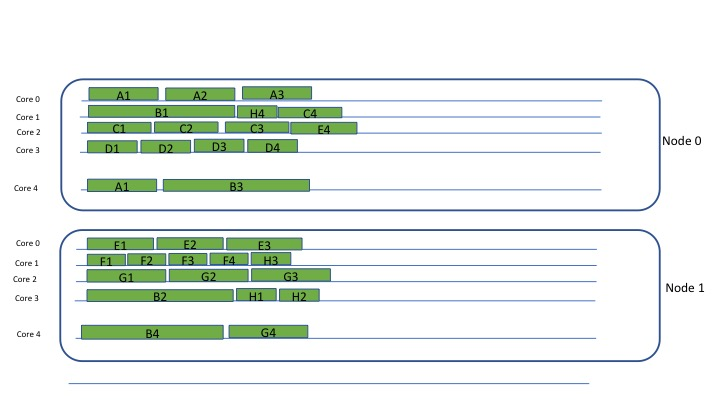
\includegraphics[width=0.75\columnwidth]{./images/CharmLdbWithLoop-manyChares}\\
      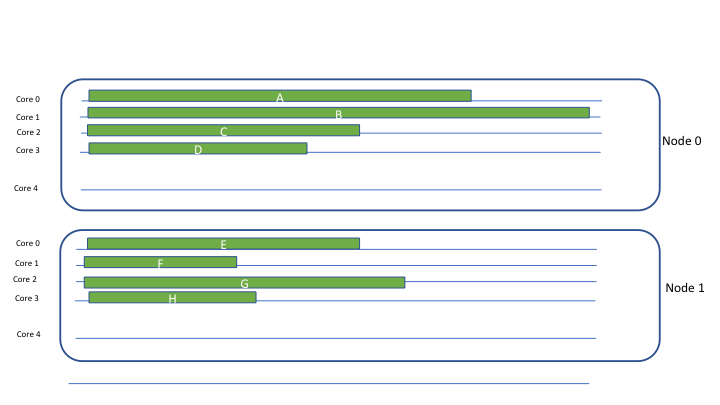
\includegraphics[width=0.75\columnwidth]{./images/CharmLdbWithLoop-fewChares}
      \label{fig:charmcklooptimeline}
    \end{center}
    \caption{\label{fig:charmcklooptimeline}\small Timelines using Charm++-only for default (left) and a mode where the number of chares per node\\ is reduced (right). }
    %Each green rectangle corresponds to execution of a Charm++ object on a core.            
  \end{figure}
\end{column}
\end{columns}
\end{frame}

\begin{frame}{Using Existing Intelligent Strategies for Internode Load Balancing}
\begin{columns}
\begin{column}{0.5\textwidth}
\begin{itemize}
\small \item \small The loop parallelism must handle dynamic imbalances while preserving locality.
\item \small The mixed static/dynamic scheduling previously developed is a promising scheduling strategy for this purpose.
\item \small A solution using only within-node loop scheduling won't handle inter-node load balance that's significant in many applications.
\end{itemize}
{\small $\rightarrow$ Need to modify load balancer so that it uses loop scheduling and is adjusted to reduce overhead of load balancing.}
\end{column} 

\begin{column}{0.5\textwidth}
\begin{figure}[ht!] \label{fig:charmBeforeAndAfterLdBCkLoop}
  \begin{center}
    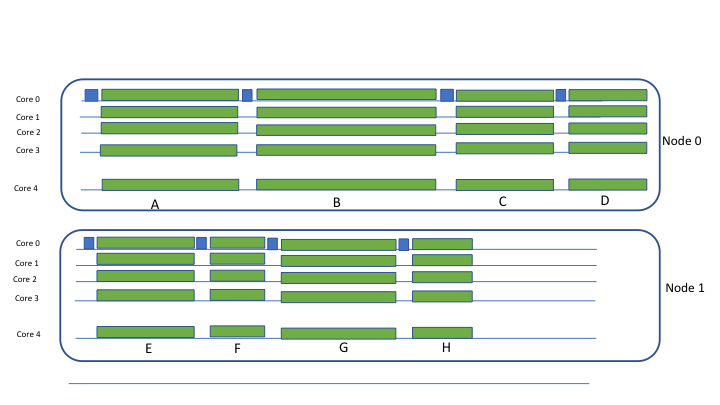
\includegraphics[width=.8\columnwidth]{images/charmLdbWithLoopwCharmonly-unbalanced}\\
    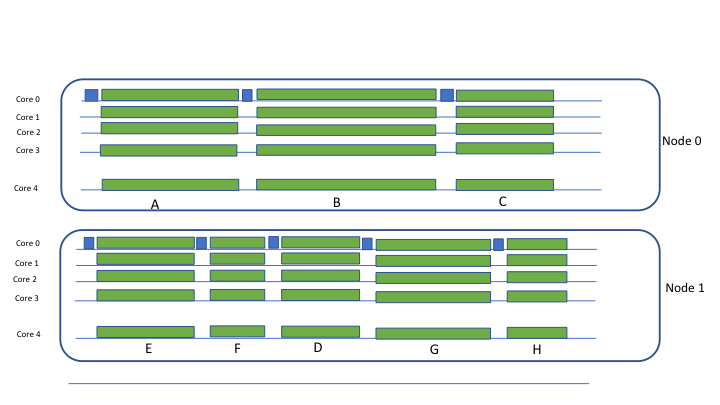
\includegraphics[width=.8\columnwidth]{images/charmLdbWithLoopwCharmonly-balanced}
  \end{center}
  \caption{\label{fig:charmBeforeAndAfterLdBCkLoop} \small Timelines for execution of a code without (left) and with (right) Charm++ load balancing.}
  %\\ A green rectangle on a non-zero core on a node corresponds to loop iterations spawned from core 0. 
\end{figure}
\end{column}
\end{columns}
\end{frame}

\begin{frame}{Key Idea of Our Solution}
\begin{columns}
\begin{column}{0.5\columnwidth}
\begin{enumerate}
 \item Modify Charm++ RTS to assign chares to core 0 of each node only.
 \item Reduce the number of chares per PE.
 \item Adjust parameters of within-node loop scheduler,e.g., vary
  static fraction, based on parameters of Charm++. 
\item Tune Charm++ RTS parameters to work with adjustments of within-node loop scheduling.
\end{enumerate}
\end{column}
\begin{column}{0.5\columnwidth}
  \begin{figure}
    \label{fig:statDynSched}
    \begin{center}
      \subfloat[\tiny Static Scheduling.]{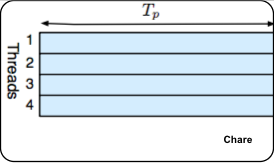
\includegraphics[width=.20\columnwidth]{./images/threadedCompRegion-static-withChare}}\hspace*{0.1in}
               \subfloat[\tiny Dynamic Scheduling.] {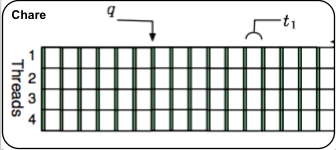
\includegraphics[width=.27\columnwidth]{./images/threadedCompRegion-dynamic-withChare}}\hspace*{0.1in}
                        \subfloat[\tiny Mixed Scheduling] 
 {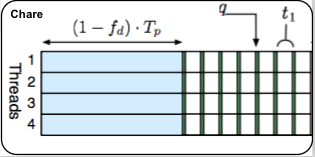
\includegraphics[width=.24\columnwidth]{images/threadedCompRegion-hybrid-withChare}}
    \end{center}
    \caption{\label{fig:statDynSched} \tiny Mixed static/dynamic scheduling within a chare, i.e., a
      Charm++ object.}
  \end{figure}
\end{column}
\end{columns}
\end{frame}

\begin{frame}{Baseline Results and Analysis}{Existence of Within-node Load Imbalance through Heat Maps}
\begin{figure}[ht!]
\begin{center}
{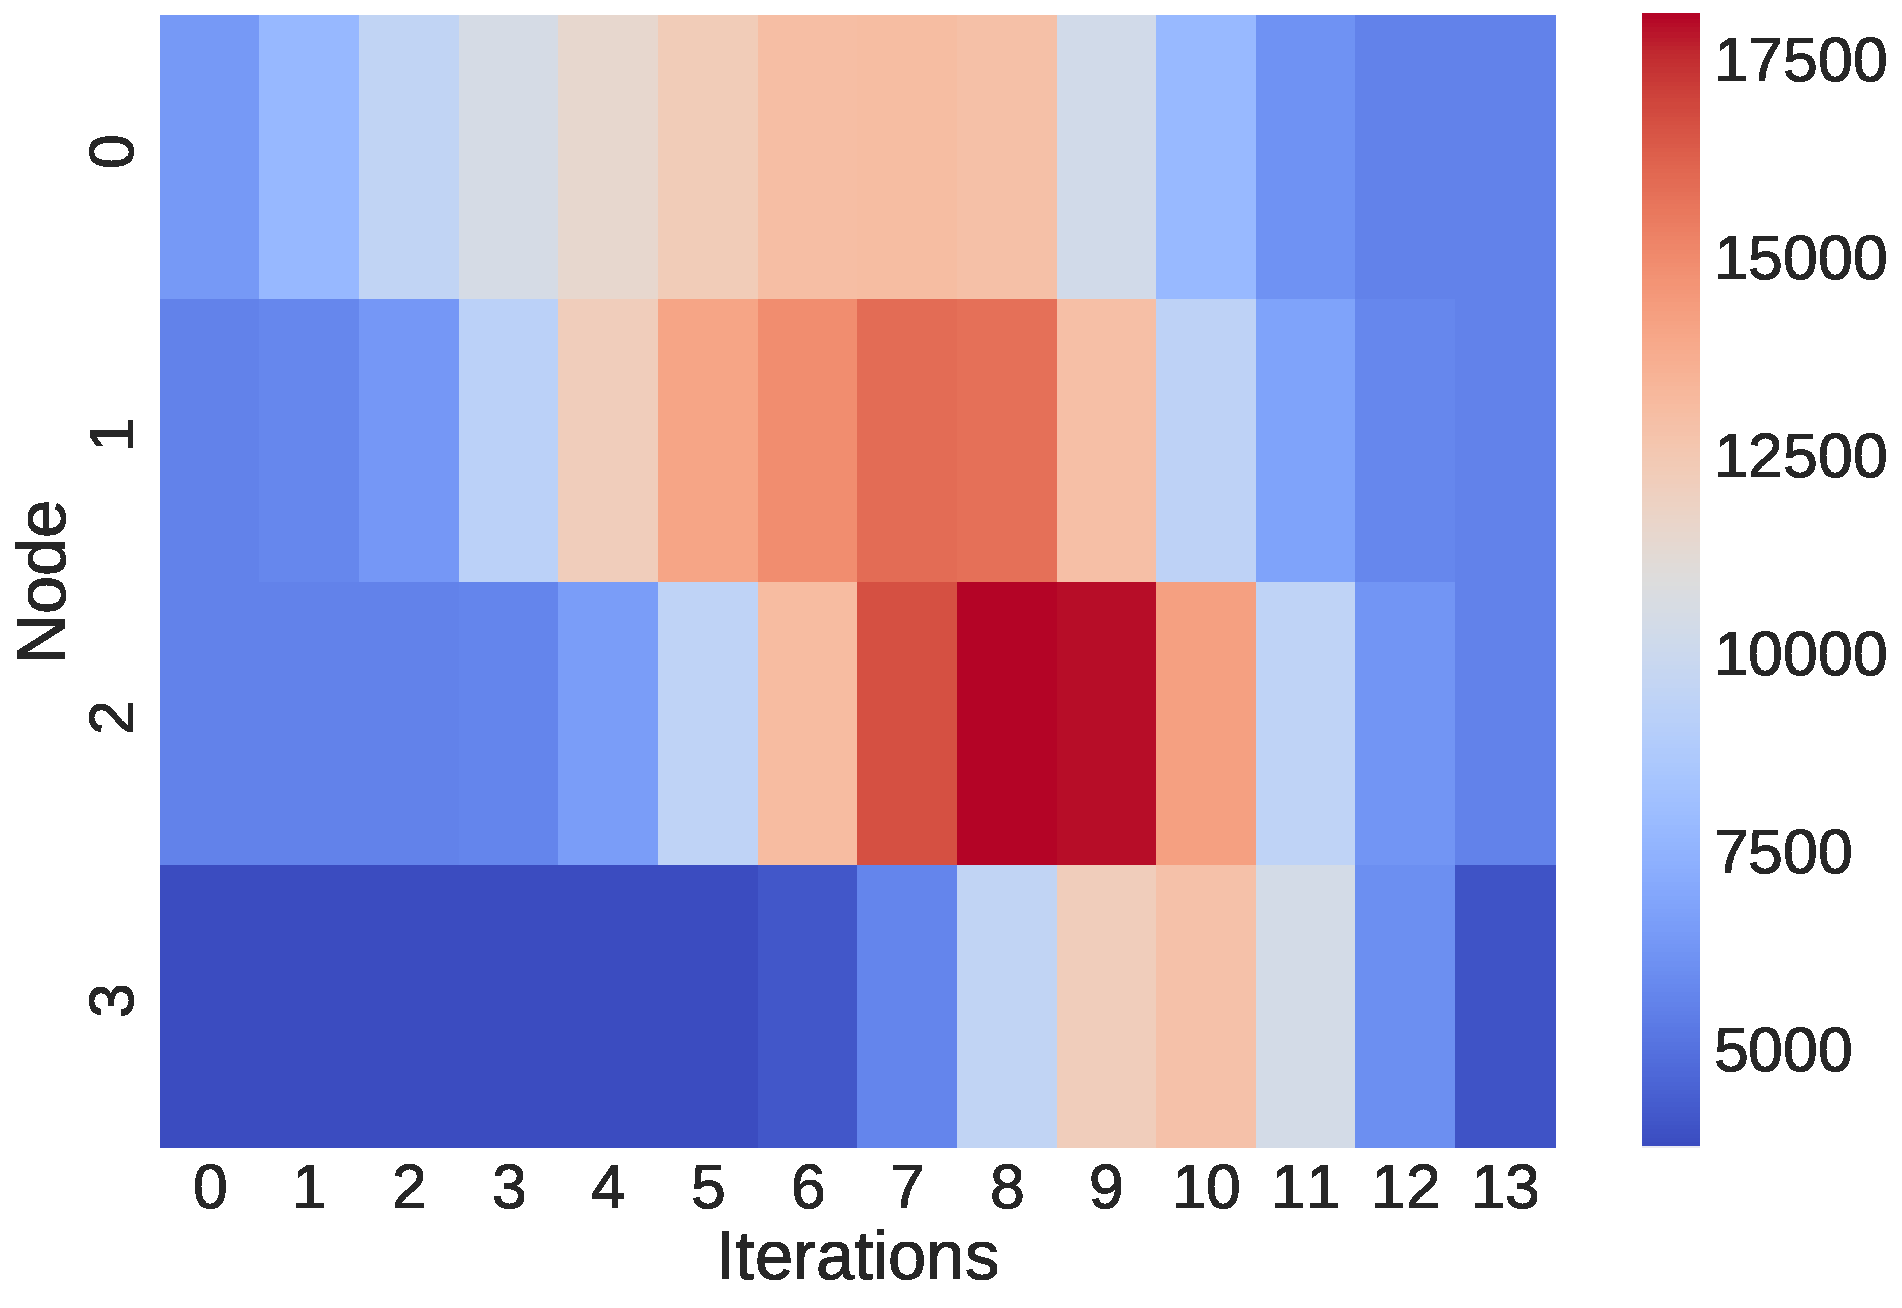
\includegraphics[width=.25\columnwidth]{images/nolb_node_load_with_iter}}
{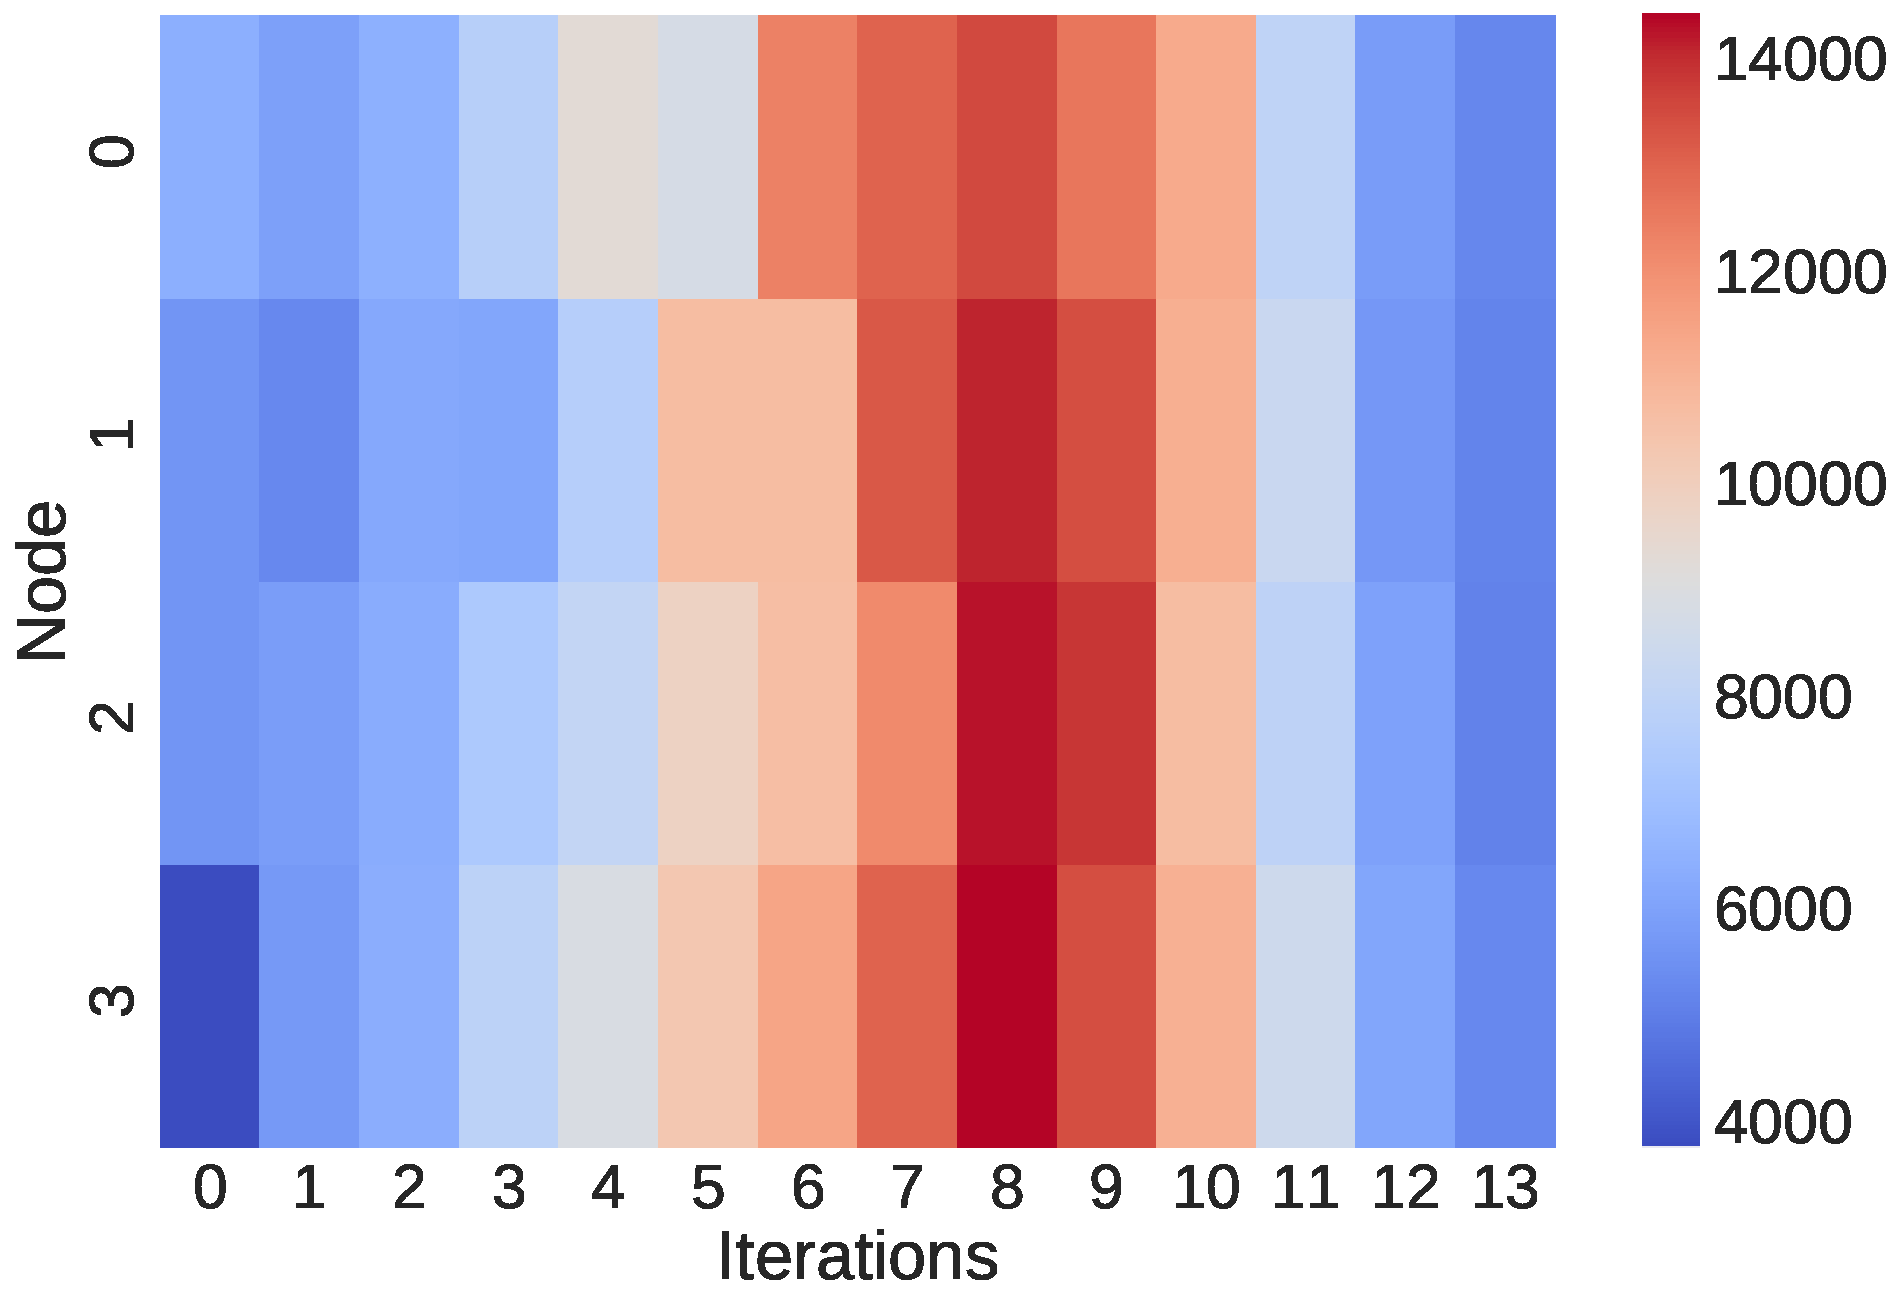
\includegraphics[width=0.25\columnwidth]{plots/greedylb_node_load_with_iter__2_.pdf}}\\
{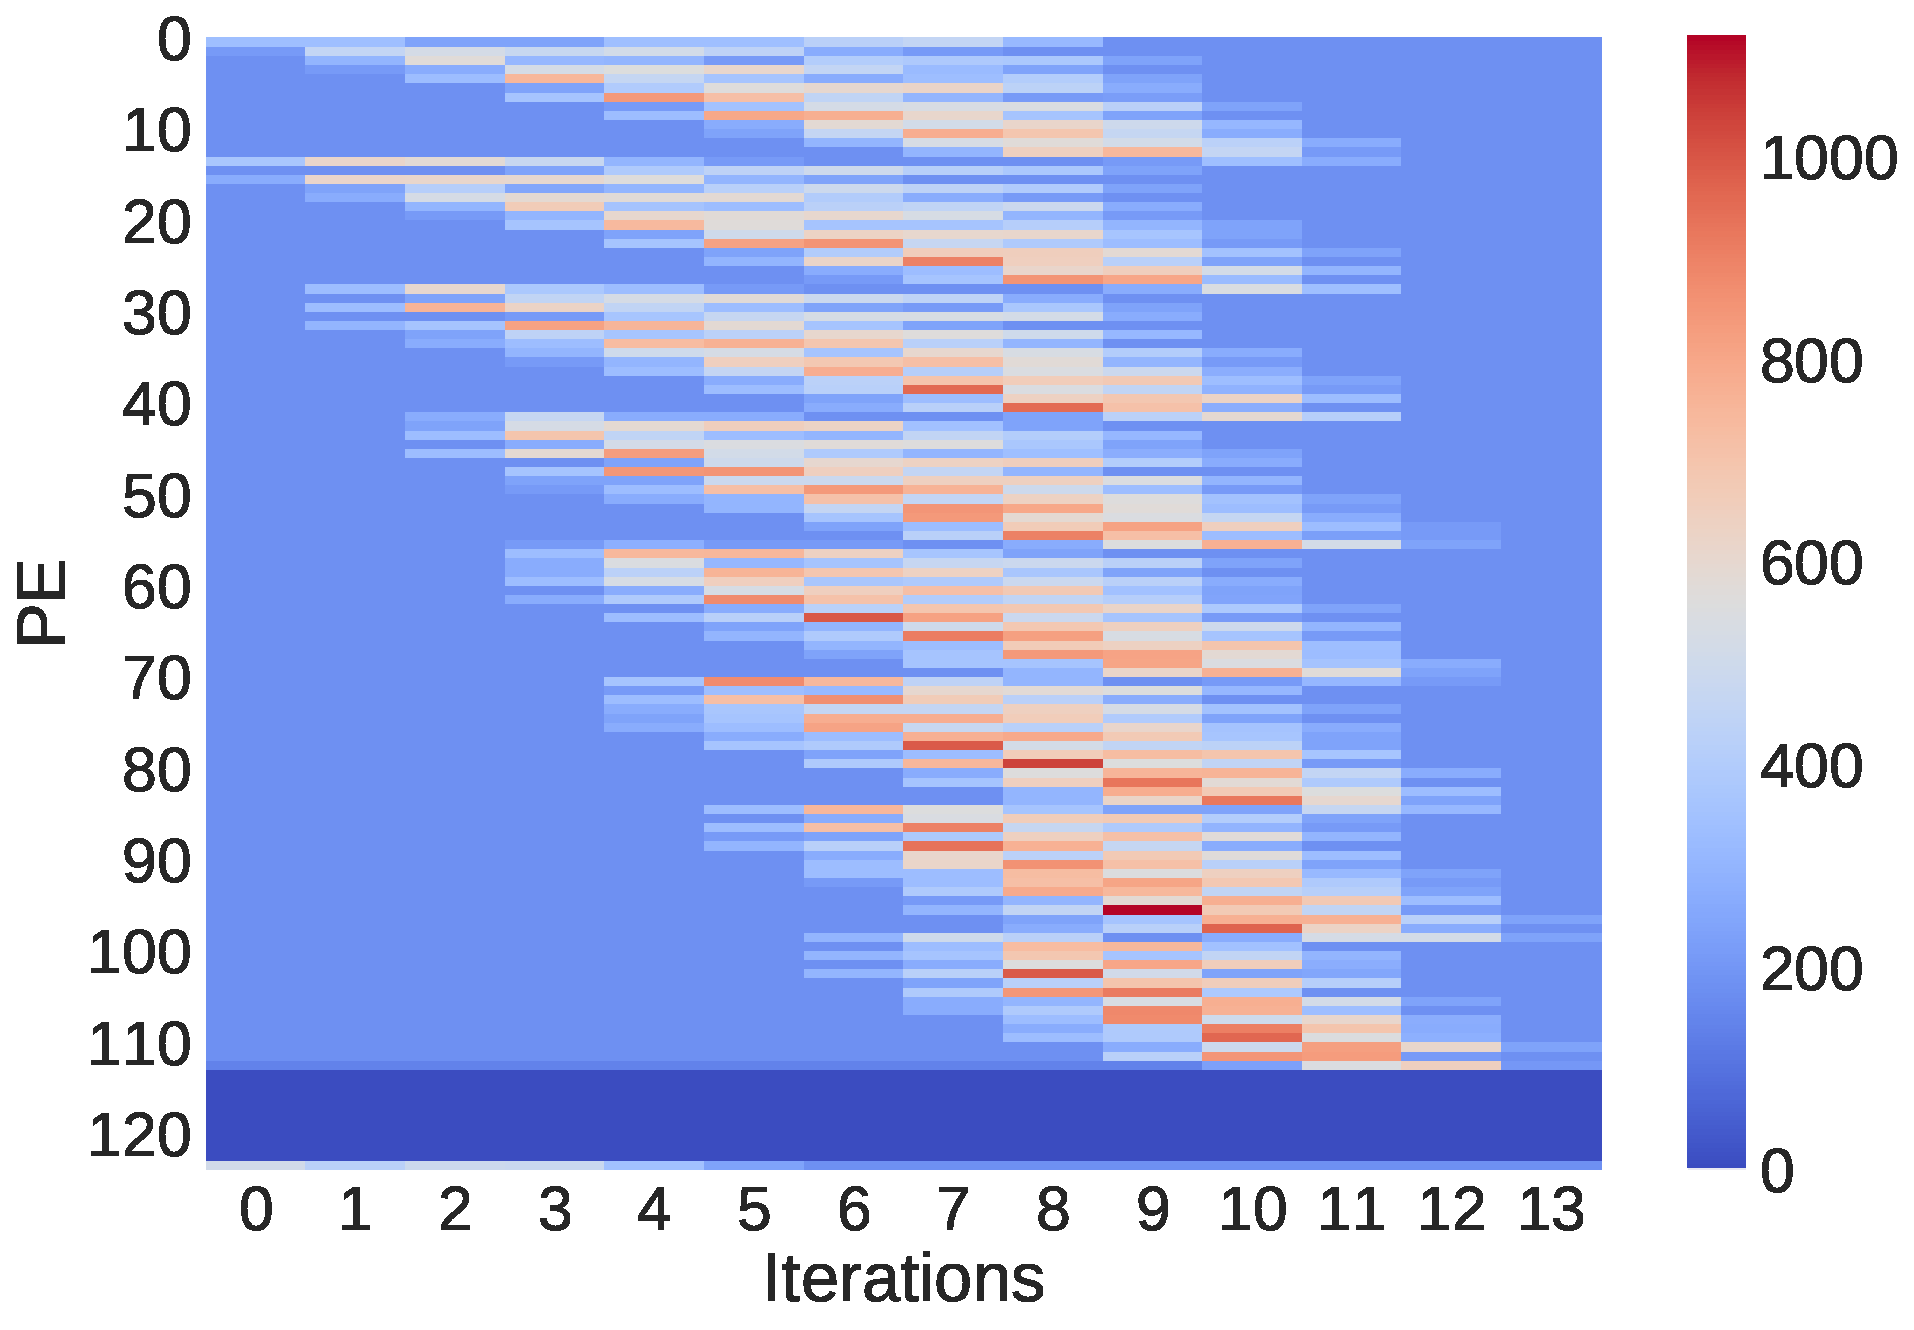
\includegraphics[width=0.25\columnwidth]{images/nolb_pe_load_with_iter}}
{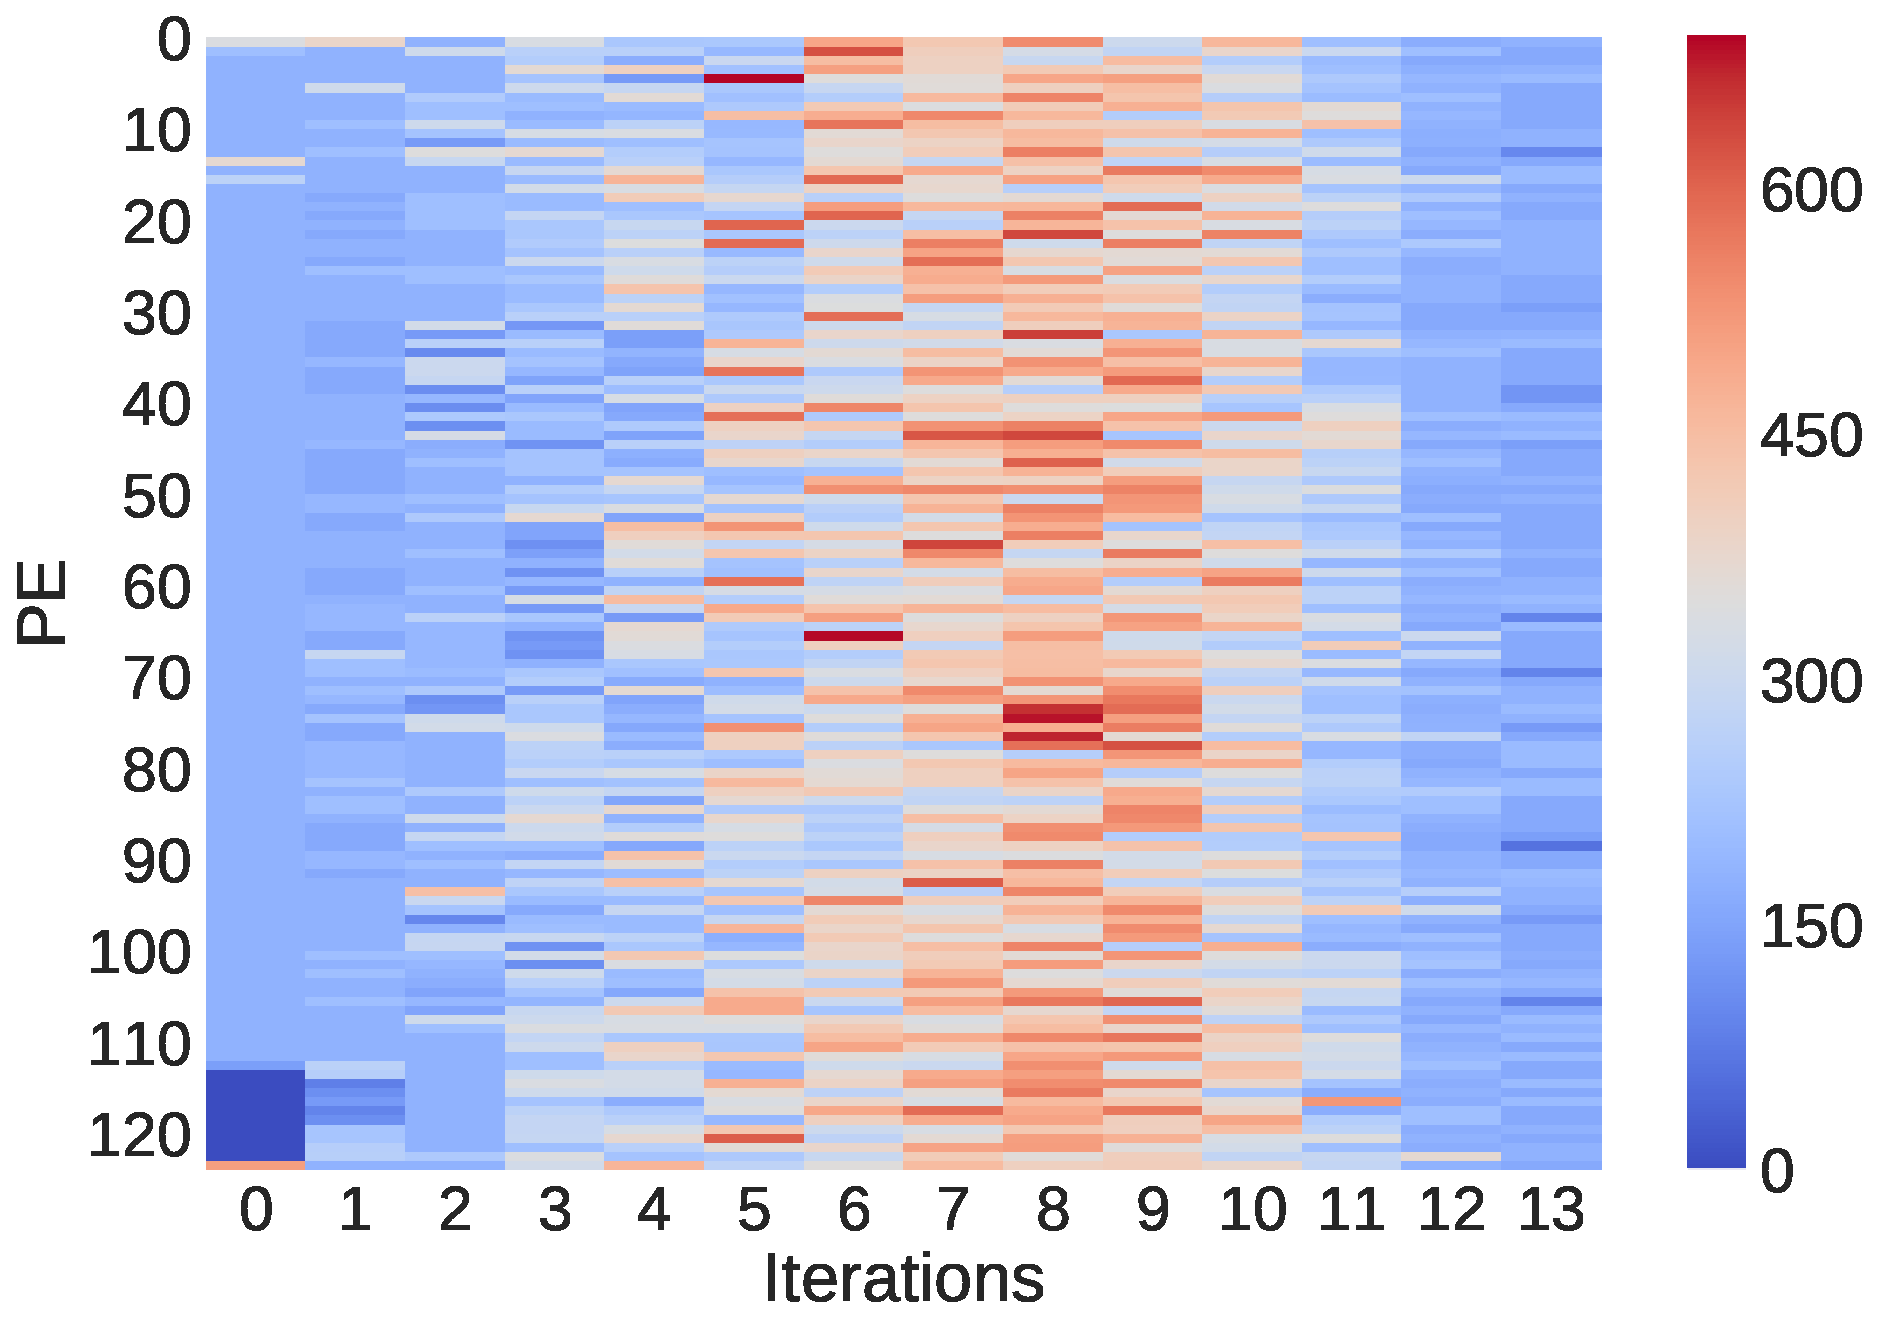
\includegraphics[width=0.25\columnwidth]{plots/greedylb_pe_load_with_iter}}
\end{center}
\caption{\label{fig:motexample2} \footnotesize Load imbalances across nodes (left) and across cores (right) when the greedy load balancing strategy is used.}
\end{figure}
\begin{itemize}
\tiny \item \tiny Using no load balancing, node 2 is heavily overloaded for iterations 8 and 9. Hence, we need load balancing to distribute the load across nodes.
\item \tiny Inter-node load balancing using GreedyLB balances load across nodes well.
\item \tiny Balancing load across nodes using GreedyLB still leaves load imbalance in the cores within a node.
\end{itemize}
\end{frame}

\begin{frame}{Additional Baseline Results}
\begin{figure}
 \label{fig:addbr}
    \centering
  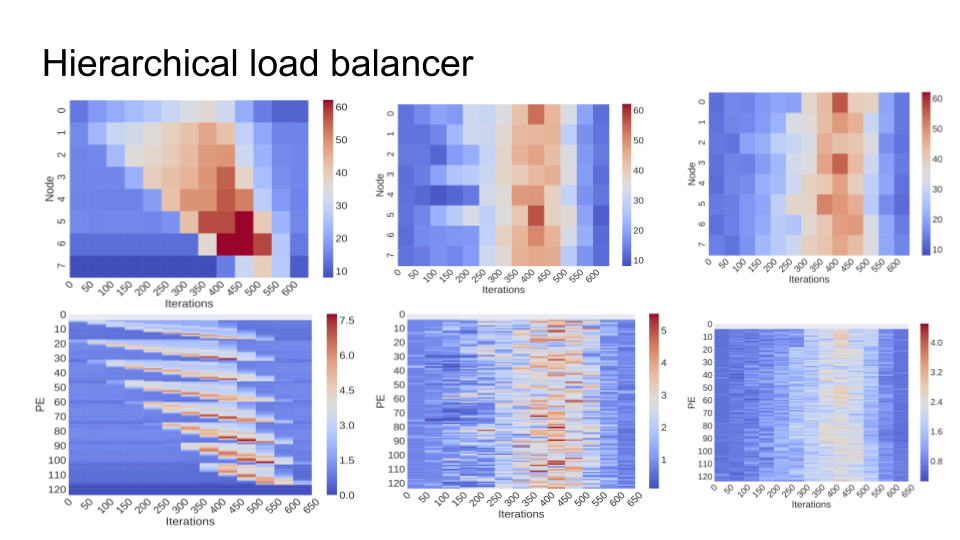
\includegraphics[scale=0.3]{plots/additionalBaselineResults.png}
  \caption{\label{fig:addbr}Baseline Results for Lassen Using Charm++ + OpenMP implementation shown in the middle.} 
\end{figure}
\end{frame}

\begin{frame}{Proposed Set of Techniques}
  \begin{enumerate}
  \item We decide on the combinations of advanced loop scheduling and advanced load balancing strategies to use. 
  \item We either experimentally tune or use an automated technique to adjust parameters of load balancing and loop scheduler together to improve performance of application. 
  \item We then consider advanced load balancing and loop scheduling strategies that can help for the combined load balancing and loop scheduling technique.
  \end{enumerate} 
\end{frame}

\begin{frame}{Performance Model for Load Balancing and Loop Scheduling}
            % first row is the table of parameters                          
            \begin{table}[h!t]
              \centering
              \label{tab:pmta}
              \begin{tabular}{|l|l|}
                \hline
                \tiny$t_1$    & \tiny Duration of a loop iteration\\ %iteration on one core \\
                \hline
                \tiny$T_p$    & \begin{tabular}[c]{@{}l@{}}\tiny Total execution time of a threaded computation region\vspace*{-0.3in} \\ \tiny consisting of $N$ loop iterations on $p$ cores\end{tabular} \\ \hline
                  %             \tiny$q$      & \tiny Scheduler's dequeue overhead of a loop iteration                                                                 \\ \hline  
                  %             \tiny$d$  & \tiny Time for executing an iteration dynamically 
                  \\ \hline
                  \tiny$\delta$ & \tiny Expected cost of load imbalance on a node to the application                                         \\ \hline
                  \tiny$load_i$ & \tiny Load on the $i^{th}$ core of a node on an arbitrary timestep                             \\ \hline
              \end{tabular}
              \caption{\label{tab:pmta} \tiny Terms in implementation}
            \end{table}
\end{frame} 

\begin{frame} 

\begin{itemize} 
\item We refer to this scheduling strategy as \emph{adaptive loop scheduling} and use a parametrized version of it to schedule loop iterations of a chare to cores. 
\item The best-performing collection of scheduler parameter values is the best-performing one, on average, for each chare. An optimal collection of scheduler parameter values, in isolation, isn't necessarily the best-performing, given an arbitrary collection of parameter values for the load balancer. 
\item Thus, our technique is to search for the collection of parameter values for the scheduler together with those for the load balancer that obtains best performance.
\end{itemize} 

\end{frame} 


\begin{frame}{Technique} 

\begin{columns}
\begin{column}{0.5\columnwidth}
{\scriptsize \underline{\textbf{Scheduling Strategies}}}
 \begin{itemize}
 \tiny \item \tiny Mixed static/dynamic
 \item \tiny Weighted dynamic
 \item \tiny Staggered
 \end{itemize}
{\scriptsize \underline{\textbf{Load Balancing Strategies}}}\\
\begin{itemize}
\tiny \item \tiny Periodic
\item \tiny Hierarchical
\end{itemize}
\end{column}


\begin{column}{0.5\columnwidth} 
{\scriptsize \underline{\textbf{Parameters of Scheduler}}}\\
\begin{enumerate}
\tiny \item \tiny Static fraction.
     \item \tiny Chunk size.
     \item \tiny Distribution of chunk sizes in queue.
     \item \tiny Cores per steal queue.
\end{enumerate}
{\scriptsize \underline{\textbf{Parameters of Load Balancer}}}\\
\begin{enumerate}
 \tiny \item \tiny Chares per PE.
 \item \tiny Frequency of load balancing step.
           % TODO: word the bullet above better
\end{enumerate}  
\end{column}
\end{columns}
         \begin{figure}[ht!]
           \label{fig:charm++locopthybsched}
           \begin{center}
             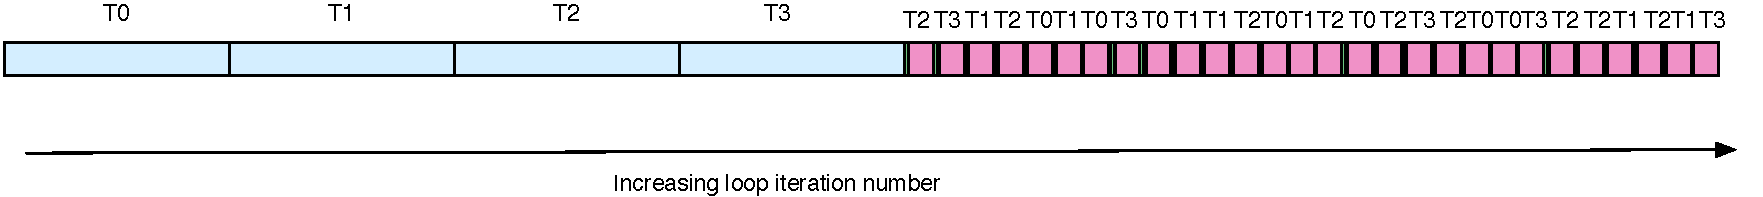
\includegraphics[scale=0.2]{./images/sdIncrIters}\\
             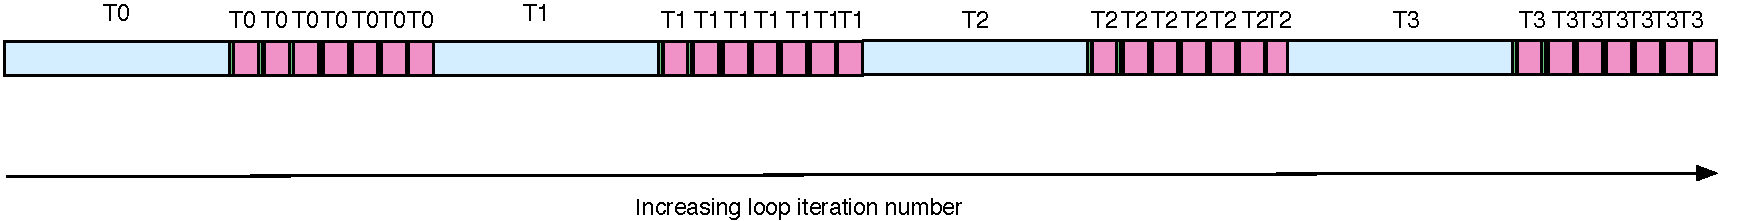
\includegraphics[scale=0.2]{./images/sdsIncrIters}
           \end{center}
           \vspace*{-0.1in}
           \caption{\label{fig:charm++locopthybsched} \tiny Mixed static/dynamic scheduling using an optimization of iteration staggering}
         \end{figure} 
         
         {\scriptsize \underline{\textbf{Methodology for Tuning Parameters}}}
         \begin{itemize}
               \tiny \item \tiny The parameters of the load balancer and of the scheduler can't be tuned independently.
             \item \tiny We tune the parameters of the scheduler and load balancer together.
         \end{itemize} 
   \end{frame} 
   
\begin{frame}{Advanced Load Balancing Techniques} 
\begin{itemize}
\item A hierarchical strategy for load balancing
\begin{itemize}
\item Frequent intra-node load balancing.
\item Infrequent inter-node load balancing.
\end{itemize}
\item Inter-node load balancing strategy would distribute work load taking into account
\begin{itemize}
\item Topology aware
\item GPU + CPU hybrid architecture
\end{itemize}
\item Use machine learning techniques to decide the most suitable strategy to use.
\end{itemize}
\end{frame} 

   
   
\begin{frame}{Loop Scheduling Techniques}
The following loop scheduling techniques will be beneficial in the
context of this work.
\begin{itemize}
\item Tapering:
\begin{itemize}
\item Useful for workloads with irregular load imbalances
\end{itemize}
\item Weighted dynamic.
\begin{itemize}
\item Helpful when certain cores within a node are slow.
\item Uses ideas of measurement-based load balancing
\end{itemize}
\item Tuning task gain size distribution.
\begin{itemize}
\item Helpful when certain cores have irregular load imbalances
\item Can adjust scheduler parameters based on across-node load balancing parameters.
\end{itemize}
\item Locality-aware constrained loop scheduling.
\end{itemize}
\end{frame}

%\bbi\item Bullet 1\onslide<2->{\item Bullet %2}\onslide<3->{\item Bullet 3}\onslide<4->{\item %Bullet 4}\ei

\begin{frame}{Implementation}{Overview of Software Architecture}
\begin{figure}[ht!]
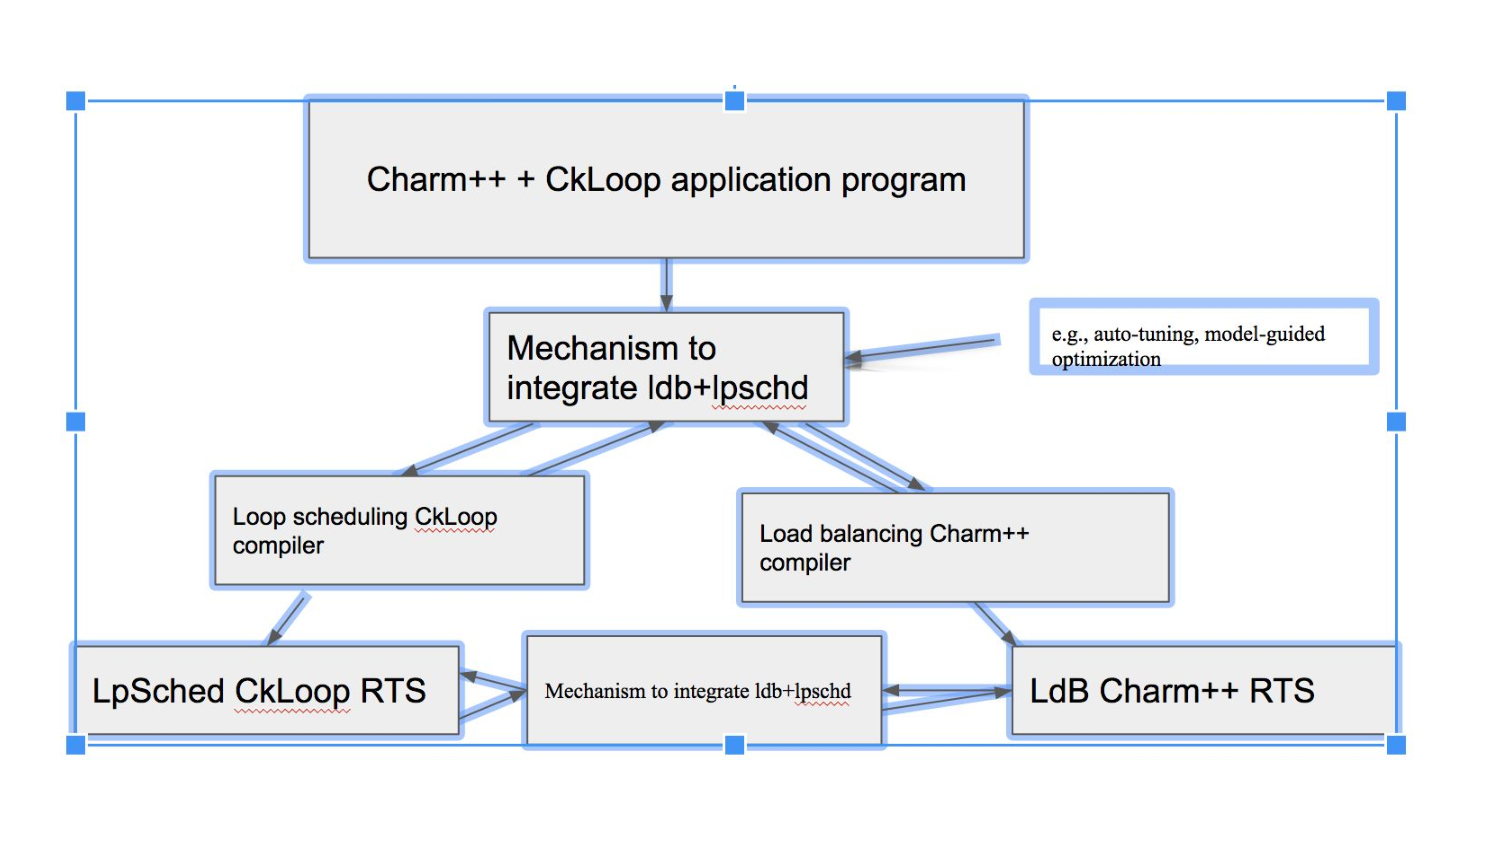
\includegraphics[scale=0.4]{./images/lslb_softwarediagram}
\caption{Diagram of Software Infrastructure for Load Balancing and Loop Scheduling Technique}
\end{figure}
\end{frame}

%\noindent {\bf Using the Modified Charm++ RTS}
\section{Modified Charm++ RTS}

\begin{frame}{Usage of Library}
%\sloppy
%\subsubsection{Usage of Library}
%in the lines of code.
\vspace*{-0.1in}
\begin{figure}[h!t]
%\begin{center}
%\lstinputlisting{./listings/dotpcharmckhyb-short.cc}
%\vspace*{-.2in}
%\caption{{\label{code:dotpcharmckhyb}User code for dot product implemented in Charm++ with {\tt CkParLoop()}.}}
%\end{center}

    \label{code:dotpCharmckhyb}
   % \lstinputlisting{./listings/old-dotpcharmckhyb.cc}\hspace*{-1.9in}
    \vspace*{-0.8in}\caption{\label{code:dotPCharmckhyb}{\tiny  \label{code:dotpCharmckhyb} Dot product code's modification using Charm++ with CkLoop.}}
 
\end{figure}

\begin{itemize} 
\tiny  \item \tiny Figure~\ref{code:dotpcharmckhyb}
shows the user code with the adapted CkLoop library using the function {\tt CkParLoop()} for the computational region of the program.
\item \tiny The user creates a kernel for the computation region and replaces the region with a call to {\tt CkParLoop()} having the name of the kernel for the computation region as a parameter to the function.
\item \tiny Here, the user calls the function on thread 0 providing the kernel to be called, the range of iterations of the loop and the number of chunks used in the loop. 
\item \tiny The user specifies a loop history variable that has a field for the static fraction within it. 
\item \tiny The lines of code in the user code with the library is 3\% more than the original user code.
\end{itemize} 
\end{frame} 


\comments{
\begin{frame}{Implementation}{Front-end Code}
     % \vspace*{1.3in} 
     % TODO: make this subtly clear in the poster paper - a reviewer of this poster or a possible subsequent paper of this work may ask, 'why don't you do runtime adjustment of parameters or model-guided optimization?' Answer: model-guided optimization is challenging to do for an n-body simulations because of the difficulty in mathematical formulation of application's computat\
     %ion cost. For runtime adjustment, we don't want to formulate a solution prematurely.  
     % We choose experimental performance tuning to further understand our problem and develop a more sophisticated solution later. 
  \begin{figure}[h!t]
    \label{code:dotpCharmckhyb}
    \lstinputlisting{./listings/old-dotpcharmckhyb.cc}\hspace*{-1.9in}
    \vspace*{-0.8in}\caption{\label{code:dotPCharmckhyb}{\tiny  \label{code:dotpCharmckhyb} Dot product code's modification using Charm++ with CkLoop.}}
  \end{figure}
\end{frame}  
}
%\begin{frame}{Implementation}{Back-end Code Design}
%\end{frame}

\begin{frame}{Implementation of Library}
\begin{itemize}

\small \item \small When {\tt CkParLoop()} is invoked on core 0, our scheduler enqueues a message in every core's queue describing the loop. 
\item \small Each core enqueues its dynamic iterations into its own stealable task queue and then executes its static chunk by calling the user-supplied kernel function. 
\item \small It then executes dynamic tasks from its own stealable queue and then randomly steals from other cores' queues.
\item \small The synchronization for loop termination and handling of reduction variables is also part of the implementation.
\item \small  Charm++'s scheme to allocate chares, i.e., objects, to cores was modified so that objects are initially assigned to core 0 of each node. 
\item \small The dynamic load balancer was modified to measure the loads of objects correctly in presence of the scheduler and to ensure that objects weren't re-assigned to cores other than core 0.
\end{itemize}
\end{frame} 


%\begin{frame}{Implementation of CkLoopHybrid}
%\begin{itemize} 
%\item 
%\item 
%\end{itemize} 
%\end{frame}

\begin{frame}{Experimental Setup}
   \underline{Applications}\\ 
   \begin{enumerate} 
   \item {\bf dot Product:}
   \item  {\bf PIC:} not much load balance.
  \item {\bf Lassen:} Can make modifications to the code easily and will be a good benchmark 
  \item {\bf Barnes Hut}
  \end{enumerate} 
  \underline{Setup of Compiler and Runtime}\\
  \begin{enumerate}
      \item Use default compile time options, i.e., {\tt -O3}
      \item Run with drone mode , i.e., one chare per node. 
  \end{enumerate} 
  \underline{Architectures} \\
  \begin{enumerate}
  \item \textbf{BlueWaters}:
  \item \textbf{Cori}:
  \end{enumerate} 
%  3D stencil with dynamic load imbalance injected: need to simply download from repository and insert CkLoopHybrid in it. 
  % contrary to earlier email discussion that it wouldn’t be worth it. 
\end{frame}


\begin{frame}{Results}
\begin{figure}[ht!]
          \begin{center}
            \subfloat[\tiny Dot Product on 4 nodes of Stampede.]{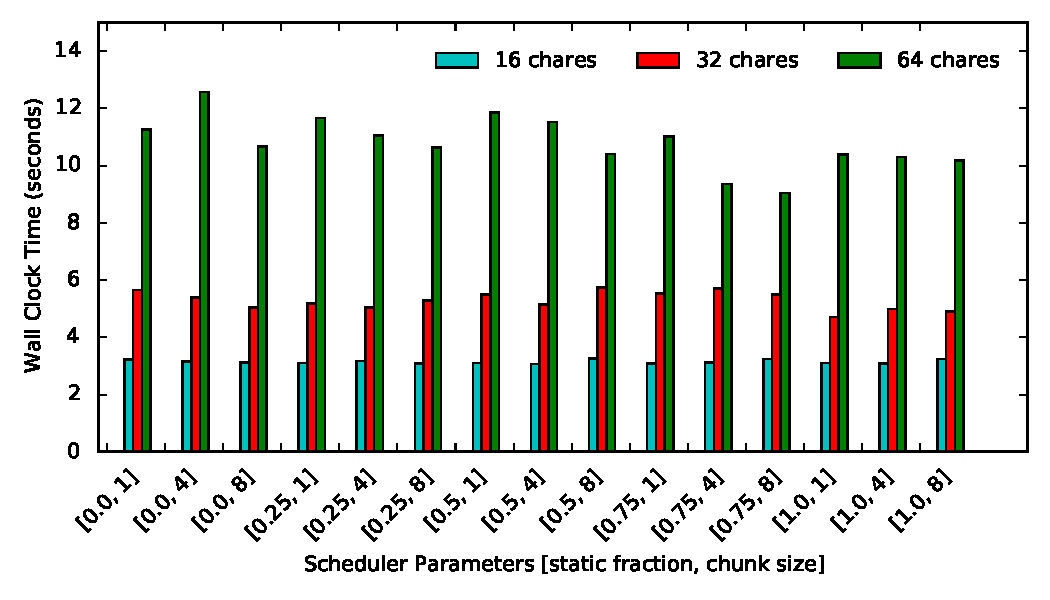
\includegraphics[width=.45\columnwidth]{plots/dotProd-4nodes-bw}} %TODO: replace with dot product results
            \subfloat[\tiny Particle-in-Cell on 4 nodes of Blue Waters.]{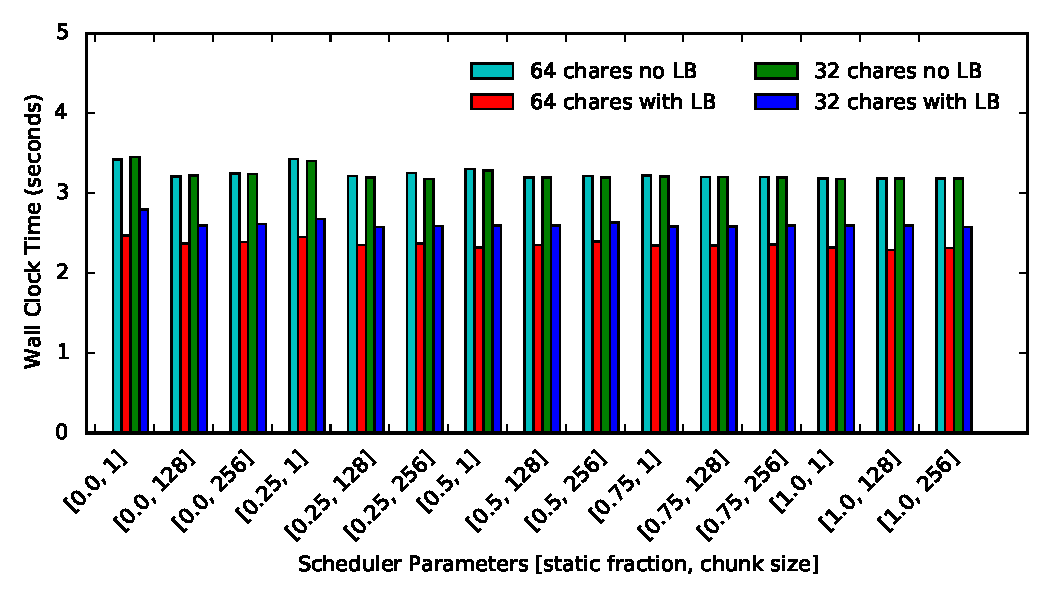
\includegraphics[width=.45\columnwidth]{plots/PIC-4nodes-bw}}
          \end{center}
          \caption{\tiny Execution times of scientific applications on multi-core clusters.}\label{fig:scalability-results-PIC-BW}
        \end{figure}
        
        
%\begin{figure}[ht!]
%\label{fig:resultsLSB}
%  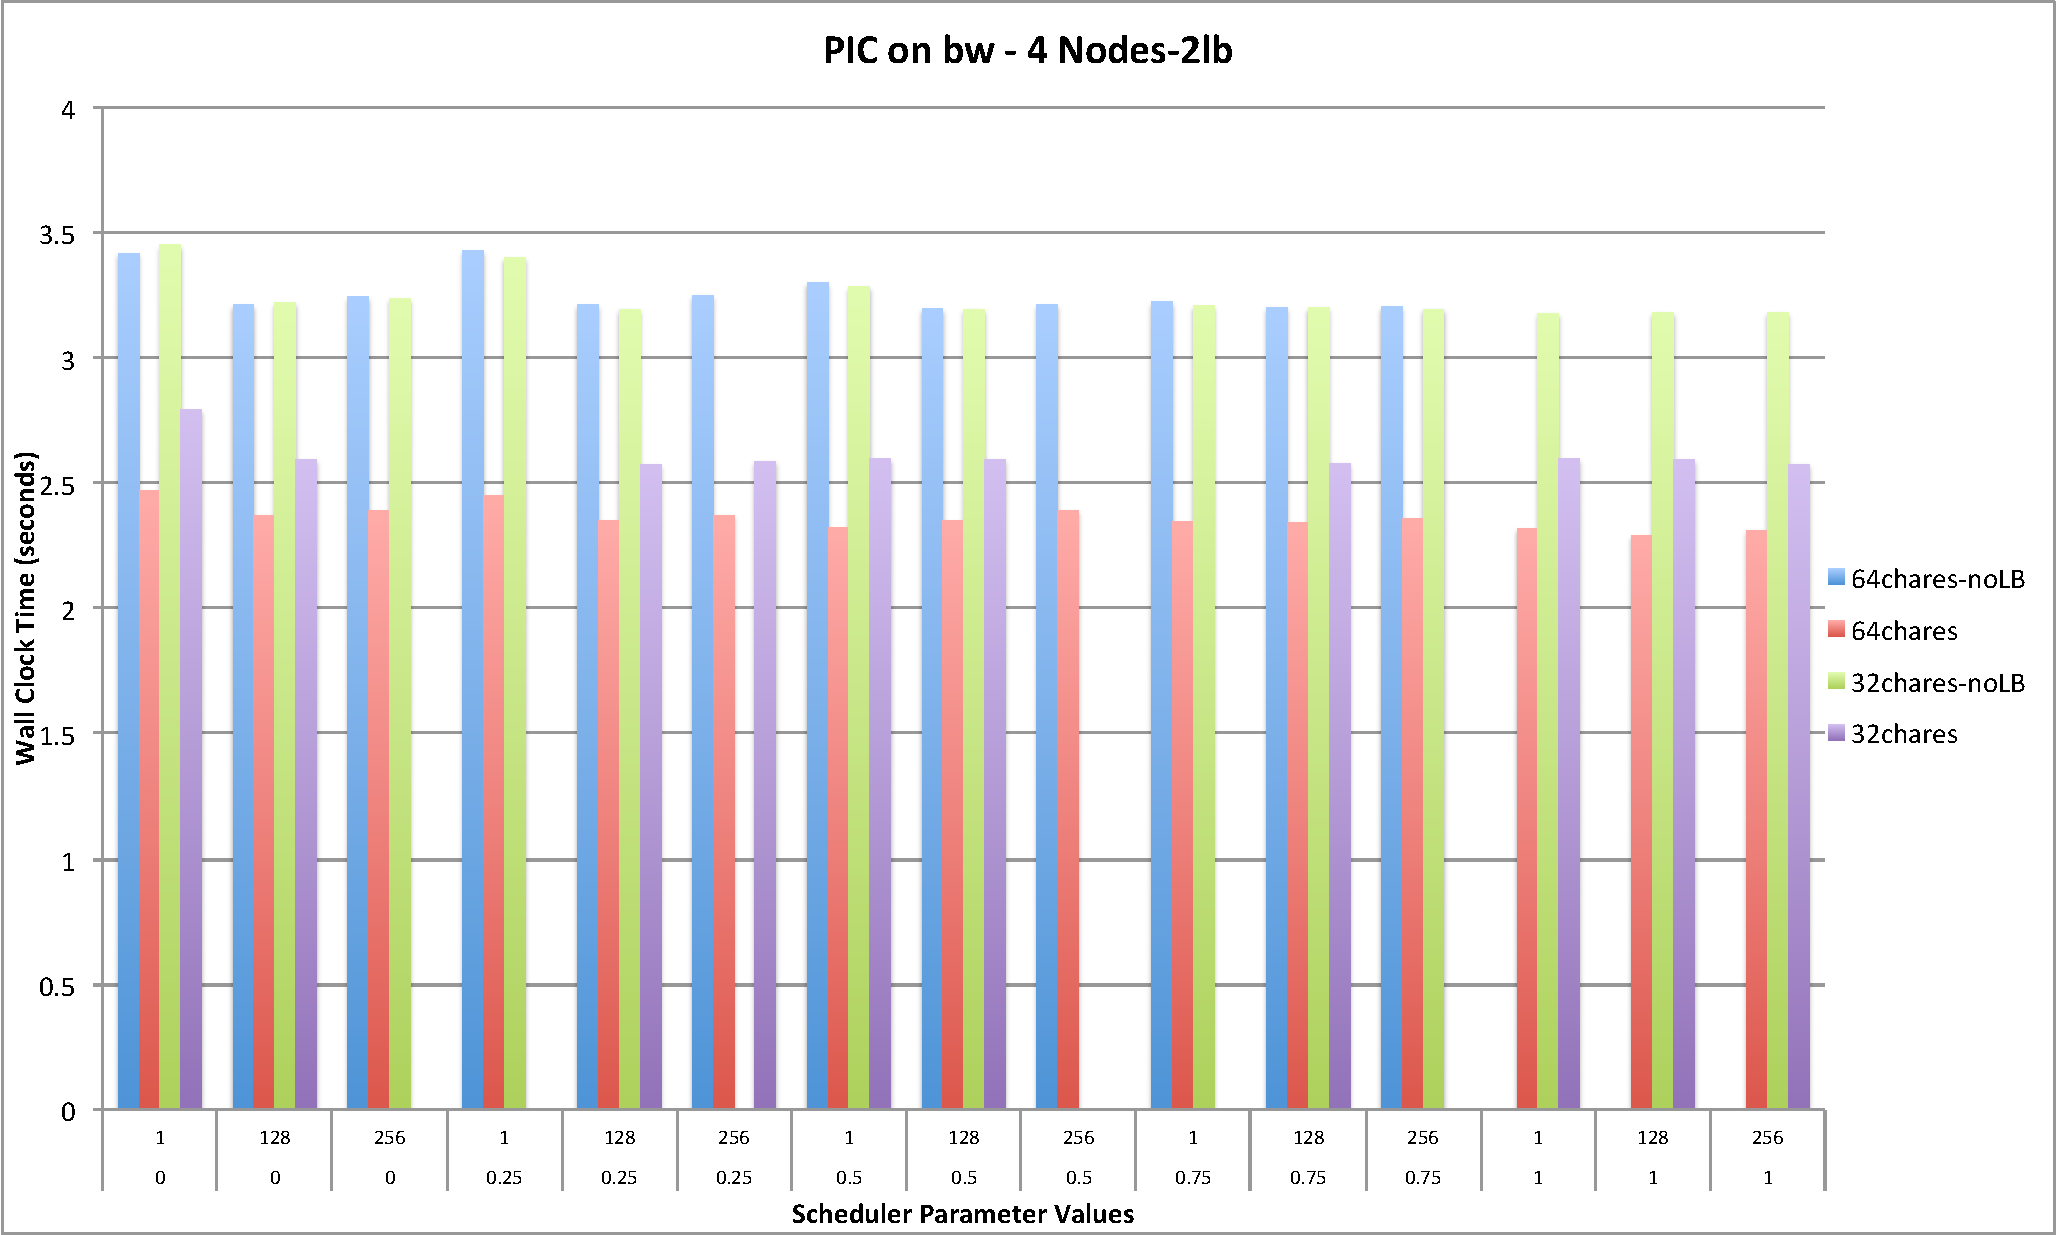
\includegraphics[scale=0.25]{plots/PIC-BW-4nodes-2lb.pdf}
%    \caption{\label{fig:resultsLSB}\small Results of using combined loop scheduling and load balancing approach in a Charm++ + CkLoop program.}
%\end{figure}

\begin{itemize} 
\item \tiny For dot product using 64 chares, a static fraction of 75\% with a chunk size of 8 gives the best performance, showing utility of adaptive loop scheduling.
\item \tiny PIC using modified inter-node load balancing with adaptive loop scheduling is 19.13\% faster than PIC using adaptive scheduling without load balancing.
%\item \tiny The percentage improvement over the original Charm++ + CkParLoop is 17.20\%.
%TODO: Fix the sentence below further to make clear what is going on. 
\item \tiny Synergistic performance improvements using combination of inter-node and intra-node load balancing. 
\end{itemize} 
\end{frame}

\begin{frame}{Related Work} 
\begin{itemize}
    \item Habanero\cite{}: library with support for data locality within node 
    \item MPI+OpenMP\cite{}: basic hybrid parallel programming model.
    \item OmpSS\cite{}: library for extensible loop scheduling schemes.
\end{itemize}
\end{frame}


\begin{frame}[label=lsbconcl]{Conclusion}{Load Balancing and Loop Scheduling}
\begin{enumerate}
\tiny \item \tiny Need sophisticated loop scheduling in Charm++. 
\item \tiny Described a technique and implementation to improve performance of applications. 
\item \tiny Using our technique and implementation, we demonstrate performance improvement \\ of 17.2\%.
\item \tiny For future work, we'll explore other adjustments to parameters of the Charm++ RTS to facilitate for loop scheduling. 
\end{enumerate} 

\end{frame}